
\documentclass{report}

\input{preamble}
\input{macros}
\input{letterfonts}

\title{\Huge{Letteratura}\\Caberlotto Giovanni}
\author{\huge{Sistemi Informativi Aziendali}}
\date{}

\begin{document}

\maketitle
\newpage% or \cleardoublepage
% \pdfbookmark[<level>]{<title>}{<dest>}
\pdfbookmark[section]{\contentsname}{toc}
\tableofcontents
\pagebreak

\chapter{La seconda metà dell'ottocento} % (fold)
\label{chap:La seconda metà dell'ottocento}

\subsection{La storia}
\subsubsection{Dal colonialismo all'imperialismo}
\\
Nella seconda metà dell'Ottocento, Gran Bretagna e Francia, seguite da Belgio, Germania e Italia, furono protagonisti della fase del colonialismo, conquistando vaste regioni in Asia e Africa. In Asia, la penetrazione europea in Cina e India segnò l'inizio dell'espansione coloniale, con la Gran Bretagna che permise un limitato autogoverno coloniale, creando i "dominions." Nel frattempo, la Francia penetrò in Indocina. L'Olanda e la Spagna erano anche presenti in Estremo Oriente, ma l'impero coloniale spagnolo era in declino già dal Settecento, e gli Stati Uniti sottrassero il dominio delle Filippine nel 1898.
\\
\\
L'Italia, entrata marginalmente nel colonialismo per motivi di prestigio, avanzò pretese sull'Africa orientale, occupando l'Eritrea e la Somalia. Nel Novecento, colonizzò la Libia (1911-1912) e l'Etiopia (1935). Questo periodo segnò il passaggio dal colonialismo all'imperialismo, caratterizzato dal totale asservimento dei Paesi coloniali alle grandi potenze impegnate nella competizione mondiale. La spartizione coloniale dell'Africa, avvenuta dopo l'abolizione della schiavitù (1833) e della tratta degli schiavi (1844), ebbe luogo nella conferenza di Berlino (1884-1885), ignorando le diversità culturali e linguistiche delle popolazioni africane. L'obiettivo era acquisire materie prime per il commercio europeo, e questa spartizione contribuì agli avvenimenti che precedettero la Prima guerra mondiale.
\\
\subsubsection{L'Italia unita}
\\
Il Regno d'Italia, formatosi nel marzo 1861, derivava dalla preesistente entità politica dello Stato sabaudo e contava 22 milioni di abitanti. Ereditando dinastia, statuto, parlamento ed esercito dallo Stato sabaudo, mantenne una continuità simbolica con la bandiera tricolore. Le "questioni" post-unificazione riguardavano il divario economico tra Nord e Sud, evidenziato dalla mancanza di benefici per il Mezzogiorno dall'arrivo degli italiani settentrionali.
\\
\\
La "questione romana" si risolse nel 1870 con l'occupazione di Roma, favorita dalla crisi internazionale seguita alla guerra tra Francia e Prussia. La "questione veneta" vide l'Italia sconfiggere l'Austria nel 1866, ottenendo il Veneto. Il periodo successivo vide il predominio della Sinistra storica, con leggi riformiste di Crispi e Crispi stesso al governo dal 1887 al 1896, caratterizzato dall'espansione coloniale e dall'incremento delle spese militari.
\\
\\
L'industrializzazione italiana, supportata dallo Stato tramite opere pubbliche e sovvenzioni, accelerò dalla fine dell'Ottocento. L'energia idroelettrica consentì alle industrie di insediarsi nelle città del Nord, ampliando il divario Nord-Sud. Lo sviluppo industriale, se da un lato portò a una crescita economica, dall'altro accentuò lo spopolamento delle campagne e la migrazione di milioni di italiani verso Nord e America Latina.
\\
\subsection{La società e la cultura}
\\
Nella seconda metà dell'Ottocento, la borghesia sostituiva gradualmente l'aristocrazia come classe dirigente, ma le monarchie europee non venivano abbattute anche con l'ascesa del liberalismo. In Francia, il conflitto centrale passò dall'opposizione tra proprietà terriera e grande capitale a una contrapposizione tra industria e finanza da un lato e proletariato e piccola borghesia dall'altro. Durante la "monarchia borghese" di Luigi Filippo d'Orléans (1830-1848), si ampliò il corpo elettorale e si stabilì un sistema parlamentare, sebbene rimanesse dominato dalla classe possidente.
\\
\nt{L'affermazione "In Francia, il conflitto centrale passò dall'opposizione tra proprietà terriera e grande capitale a una contrapposizione tra industria e finanza da un lato e proletariato e piccola borghesia dall'altro" si riferisce a un cambiamento significativo nei rapporti di potere e nei conflitti sociali durante la seconda metà dell'Ottocento in Francia.
\\
\\
All'inizio di questo periodo, c'era una contrapposizione tra la classe aristocratica e la borghesia emergente, che stava gradualmente sostituendo l'aristocrazia come classe dirigente. Tuttavia, nel corso del tempo, il conflitto centrale si spostò dalla lotta tra la proprietà terriera (rappresentata tradizionalmente dall'aristocrazia) e il grande capitale (rappresentato dalla borghesia industriale) a una nuova contrapposizione.
\\
\\
La nuova contrapposizione emersa in Francia fu tra, da un lato, l'industria e la finanza rappresentate dalla borghesia industriale e finanziaria e, dall'altro lato, il proletariato (classe lavoratrice) e la piccola borghesia. Questo riflette un cambiamento nella struttura economica e sociale del paese, con un'accentuazione delle differenze tra i detentori del potere economico e coloro che dipendevano dal lavoro per sussistere.}
\\
\\
Fuori dal Parlamento, emersero movimenti democratici, gruppi radicali e partiti che adottarono diverse forme di lotta. A metà dell'Ottocento, in tutta Europa, cresceva un vasto movimento di emancipazione, segnando un'epoca in cui le masse popolari rivendicavano diritti politici ed economici per la prima volta nella storia. Questo secolo, oltre al progresso, fu caratterizzato dal movimento operaio, organizzato attraverso partiti dei lavoratori, associazioni internazionali, società di mutuo soccorso, leghe e sindacati. Le ideologie dominanti in questo contesto furono il liberalismo e il socialismo, con lo sviluppo del pensiero marxista e del comunismo.
\\
\subsubsection{Il pensiero Marxista}
\\
Karl Marx e Friedrich Engels, pensatori tedeschi del XIX secolo, elaborarono un'analisi scientifica e rivoluzionaria della struttura economica della società. La loro visione, definita materialistica, sosteneva che le relazioni in una società sono sempre legate a una struttura economica, un modo di produzione collegato alle forme di convivenza e cooperazione. Questo legame indissolubile tra società ed economia è basato sulla contraddizione fondamentale tra forze produttive (lavoratori, mezzi di produzione, conoscenze tecniche e scientifiche) e rapporti di produzione (relazioni che regolano il possesso dei mezzi di produzione).
\\
\\
Il conflitto centrale è quello tra lavoratori e rapporti di proprietà, e questa lotta delle classi sociali per il controllo delle risorse guida le trasformazioni storiche delle società. Marx ed Engels sostenevano che la sovrastruttura giuridica e politica di una società, insieme alle forme sociali della coscienza, come diritto, religione e concezioni morali, sono prodotti della struttura economica. In altre parole, il "materialismo storico" marxista afferma che è la struttura economica a determinare gli aspetti ideologici della società, e non il contrario.
\\
\newpage
\\
\nt{Il pensiero marxista di Karl Marx ha plasmato movimenti politici globali, con radici nell'analisi del capitalismo nel XIX secolo. Nel contesto della rivoluzione industriale e degli Stati liberali emergenti, Marx ed Engels svilupparono concetti come l'alienazione, focalizzandosi sulla produzione come elemento centrale della società. Il materialismo storico di Marx attribuisce importanza cruciale all'analisi della produzione, identificando le forze produttive e i rapporti di produzione come chiavi nella definizione di un modo di produzione.
\\
\\
Marx collega le classi sociali ai rapporti di produzione, in cui la divisione del lavoro e la proprietà privata influenzano la struttura sociale. La sovrastruttura, che include politica e spiritualità, è strettamente collegata al modo di produzione, con lo Stato che preserva il dominio della classe capitalistica. Marx concepisce la rivoluzione come necessaria per rovesciare il potere borghese e introdurre la dittatura del proletariato come fase transitoria verso la società comunista senza classi e Stato.
\\
\\
Sebbene le previsioni di Marx sulla rivoluzione nei paesi industrializzati non abbiano trovato pieno riscontro, il suo pensiero continua a influenzare la comprensione critica del capitalismo e delle dinamiche sociali. Nonostante le critiche e le variazioni interpretative, l'analisi di Marx sulla produzione e i rapporti di classe rimane una risorsa chiave per comprendere le sfide sociali contemporanee.
}

\subsubsection{Il pensiero liberale}
\\
Il pensiero liberale parte dal presupposto che gli individui abbiano diritti essenziali, come il diritto alla vita, libertà e sicurezza, che lo Stato deve garantire e proteggere. Questi diritti sono considerati "naturali" e precedono l'esistenza della società, non essendo concessioni dello Stato. La Dichiarazione d'indipendenza americana e la Dichiarazione dei diritti dell'uomo della Rivoluzione francese hanno sancito la difesa irrinunciabile di tali diritti.
\\
\\
La struttura istituzionale dello Stato può variare, ma deve comunque servire e proteggere questi diritti. Il liberalismo, influenzato dall'utilitarismo di teorici come Jeremy Bentham e John Stuart Mill, considera il bene come coincidente con l'utile, ma questo utile è inteso nell'ottica del vantaggio per l'intera società, non solo per l'individuo. L'utilitarismo liberal promuove la solidarietà sociale, l'atteggiamento altruistico e umanitario. Rispetto alle correnti comuniste del XIX secolo, il liberalismo si distingue per il rifiuto dei metodi rivoluzionari, preferendo il riformismo, e per la convinzione che la libertà individuale non debba essere limitata, neanche in nome dell'uguaglianza sociale, poiché per i liberali la libertà individuale è un valore supremo.
\\
\\
\subsubsection{Differenza tra pensiero liberale e liberismo}
\\
\nt{Il liberalismo è un atteggiamento politico che sostiene la massima libertà individuale e la limitata interferenza dello stato nella vita dei cittadini. I liberali promuovono la tripartizione dei poteri per evitare concentrazioni eccessive di autorità. Il dibattito si intensifica durante eventi come il lockdown, dove la libertà personale può entrare in conflitto con l'intervento dello stato a fini di salute pubblica.
\\
\\
Il liberismo, d'altro canto, è un modello economico che si concentra sulla libera iniziativa individuale. Secondo Adam Smith, il mercato dovrebbe autoregolarsi senza interferenze statali, rappresentato dalla "mano invisibile". Tuttavia, le critiche emergono durante crisi come l'aumento dei prezzi durante la pandemia, richiedendo interventi governativi.
\\
\\
In conclusione, il liberalismo riguarda l'atteggiamento politico generale, mentre il liberismo è un modello economico che enfatizza la libera iniziativa individuale. La sfida si pone quando la libertà individuale entra in conflitto con la tutela collettiva, soprattutto durante eventi straordinari.}
\\
\subsubsection{Il progresso delle scienze e il positivismo}
\\
La fiducia nel progresso, condivisa da diverse filosofie e movimenti politici, era fondata sull'avanzamento inarrestabile delle scienze. I risultati scientifici, tangibili nella vita quotidiana, facevano sembrare il mondo più piccolo, facilitando comunicazioni e trasporti grazie a invenzioni come il motore a scoppio e il trasporto a vapore. Queste innovazioni avevano impatti diretti sulla produzione industriale e sulla qualità della vita, come nel caso della lampadina che consentiva turni serali nelle fabbriche.
\\
\\
Il passaggio dalla scienza alla tecnologia diveniva sempre più immediato, specialmente nelle scienze biologiche e mediche con le scoperte di batteriologi come Louis Pasteur e Robert Koch, che portarono alla produzione di vaccini. L'abbandono di prospettive teologiche e metafisiche a favore di un approccio scientifico e positivo caratterizzava la cultura europea. Le idee del Positivismo, soprattutto quelle di Auguste Comte, furono adottate da pensatori laici come i marxisti e i liberali.
\\
\nt{Auguste Comte (1798-1857) è stato un filosofo e sociologo francese, noto come uno dei fondatori della sociologia. La sua opera principale, "Corso di filosofia positiva," introdusse il positivismo, un approccio che sostiene che la conoscenza scientifica basata sull'osservazione empirica è la forma di conoscenza valida. Comte propose la "legge dei tre stadi," che indica lo sviluppo della società attraverso fasi teologiche, metafisiche e scientifiche. Nel "Sistema di politica positiva," estese il positivismo alla politica, proponendo un sistema sociale basato su principi scientifici. Sebbene alcune sue idee siano state criticate, il contributo di Comte alla nascita della sociologia ha avuto un impatto duraturo.}
\\
\\
Nell'Ottocento, la visione utilitaristica e solidale dell'utilità sociale si differenziò dalle correnti comuniste, orientandosi verso il riformismo. 
\\
\nt{Il riformismo rappresentava un'ideologia che propugnava il miglioramento graduale e pacifico delle condizioni sociali ed economiche attraverso riforme legislative e istituzionali. A differenza delle correnti più radicali, come il comunismo, il riformismo non mirava a un cambiamento rivoluzionario immediato della società, ma piuttosto a una trasformazione progressiva e riforme gradualiste. Gli esponenti del riformismo cercavano di apportare miglioramenti sociali attraverso ristrutturazioni legali, politiche e istituzionali, mantenendo il sistema esistente ma mitigando le disuguaglianze e migliorando le condizioni di vita dei lavoratori. Il riformismo ha avuto un ruolo significativo nei movimenti socialisti e progressisti del XIX secolo, cercando di equilibrare il progresso sociale con la stabilità istituzionale.}
\\
Charles Darwin, con la sua teoria dell'evoluzione, sconvolse le concezioni creazioniste, spiegando la comparsa di nuove specie attraverso la "lotta per l'esistenza" e la selezione naturale. Darwin riconosceva l'importanza dell'adattamento degli animali all'ambiente, in contrasto con le idee di Lamarck.
\\
\\
Il darwinismo suscitò interesse e condanne, con la possibilità di fraintendimenti politici, come la giustificazione delle disuguaglianze sociali. Herbert Spencer propose un principio di "evoluzione universale," applicato non solo alle specie viventi ma anche a ogni aspetto della realtà, con una teoria ottimistica basata sul progresso continuo, purché la lotta tra individui avvenisse liberamente, senza interventi dello Stato.
\\
\\
\nt{Jean-Baptiste Lamarck, vissuto nel XVIII e XIX secolo, fu uno dei primi teorici dell'evoluzione. La sua teoria, nota come lamarckismo, sostenne che gli organismi acquisiscono caratteristiche durante la loro vita a seguito di esperienze e che queste caratteristiche acquisite possono essere ereditate. Questa idea, ora superata, contrasta con la teoria dell'evoluzione di Darwin che si basa sulla selezione naturale. Lamarck è spesso ricordato per il suo contributo pionieristico alla comprensione dell'evoluzione biologica, anche se la sua teoria specifica è stata largamente respinta.}
\subsubsection{La questione sociale: donne, infanzia, povertà}
\\
Nel 1792, Mary Wollstonecraft scrisse "Rivendicazione dei diritti della donna", seguito da opere come "La servitù delle donne" di John Stuart Mill nel 1869. Nonostante questi sforzi, le richieste dei primi movimenti femministi impiegarono molto tempo prima di trasformarsi in riforme concrete. Il termine "suffragetta" era sinonimo di "femminista" e identificava le attiviste che lottavano per il diritto di voto femminile, riconosciuto nel mondo occidentale solo nel XX secolo.
\\
\\
Nel mondo dell'infanzia, nonostante le riforme, l'alto livello di analfabetismo e abbandono scolastico persisteva nell'Inghilterra di metà Ottocento. Nonostante le leggi sull'istruzione obbligatoria e gratuita, la povertà costringeva molti bambini a cercare lavoro in fabbrica, contribuendo alla persistenza di decine di migliaia di bambini non istruiti. Lo sviluppo industriale contemporaneo e la crisi agricola accentuavano i problemi nelle città, affollate da ex contadini e proletari in cerca di lavoro. Il sovraffollamento e la disoccupazione portavano a fenomeni come la malavita, la prostituzione, le malattie e l'emarginazione, affrontati solo parzialmente da forme di assistenza governative, ecclesiastiche, sindacali e cooperative, insieme alla beneficenza privata.
\\
\\
\nt{Mary Wollstonecraft, vissuta nel XVIII secolo, è stata una filosofa e scrittrice britannica, considerata una delle prime femministe. Nel suo lavoro più noto, "A Vindication of the Rights of Woman" (1792), ha difeso l'uguaglianza dei diritti delle donne e ha criticato l'educazione discriminatoria nei confronti delle donne. Wollstonecraft sosteneva che l'accesso all'istruzione e l'empowerment delle donne avrebbero portato a una società più giusta e progressista. La sua influenza è stata significativa nello sviluppo del pensiero femminista.}
\\
\\
\subsubsection{Voci di crisi nella cultura borghese}
\\
Nella seconda metà dell'Ottocento, il progetto politico e sociale della borghesia inizia a rivelare i suoi limiti, mettendo in discussione l'universalità delle sue rivendicazioni. Non solo i movimenti rivoluzionari, come quelli comunisti o anarchici, contestano l'orientamento liberal-democratico, ma anche il mondo della cultura, delle lettere e delle arti solleva dubbi sulla società borghese con i suoi fallimenti e paradossi.
\\
\\
Il Positivismo, con la sua scienza della società improntata ai valori della borghesia, viene criticato da poeti, pittori, compositori e romanzieri che cercano fonti di conoscenza al di fuori dei suoi confini. Artisti come Stéphane Mallarmé e Richard Wagner esplorano percorsi autonomi e alternativi, lontani dalla realtà, spingendosi verso il modernismo del Novecento.
\\
\\
\nt{Stéphane Mallarmé è stato un poeta e critico francese del XIX secolo, riconosciuto per la sua influenza nel simbolismo. La sua poesia era caratterizzata da una complessità linguistica e concettuale, con un'attenzione particolare alla musicalità e all'armonia. Mallarmé cercava di andare oltre la convenzione poetica tradizionale, sperimentando con la struttura e il significato dei versi. La sua opera più celebre è "Un coup de Dés jamais n'abolira le Hasard" (Un tiro di dadi non abolirà mai il caso), un poema visivo che sfidava le convenzioni tipografiche. La sua innovativa approccio alla poesia ha avuto un impatto duraturo sulla letteratura moderna.}
\\
\\
\nt{Richard Wagner è stato un compositore e direttore d'orchestra tedesco del XIX secolo, noto soprattutto per le sue opere musicali rivoluzionarie e l'approccio innovativo alla composizione. È considerato una figura chiave nel movimento del Romanticismo musicale. Le sue opere, tra cui "L'Olandese volante", "Tannhäuser" e la monumentale tetralogia "L'Anello del Nibelungo", hanno introdotto nuovi elementi come il leitmotiv e una visione totale del dramma musicale. Wagner era anche un teorico musicale, scrivendo estensivamente sulla filosofia dell'opera e l'importanza della "Gesamtkunstwerk" o "opera d'arte totale", che integrava musica, dramma e scenografia. La sua influenza sulla musica e il teatro è stata significativa.
}
\\
\\
Il nichilismo, rappresentato dal rifiuto estremo della realtà e dei fondamenti del pensiero borghese, emerge come forma estrema di rigetto. In particolare, nella cultura russa, scrittori come Dostoevskij e Turgenev esplorano il senso del "nulla" che tragica-mente inghiotte la possibilità di salvezza. Friedrich Nietzsche, con la sua affermazione provocatoria della "morte di Dio", proclama la fine di ogni verità, laica e religiosa, e il fallimento di ogni sistema razionale possibile.
\\
\\
\nt{Nietzsche contesta la soppressione dell'impulso dionisiaco e critica la costruzione metafisica iniziata da Platone, sostenendo che contribuisce a una visione distorta del mondo. La falsa morale derivata da questa costruzione, secondo Nietzsche, genera un rifiuto della vita. Nella sua fase successiva, annuncia la morte di Dio e introduce l'oltreuomo come risposta alla crisi culturale.
\\
\\
La filosofia del giorno propone una rinascita filosofica, in cui l'oltreuomo vive liberamente, abbracciando l'eterno ritorno e la volontà di potenza. Nietzsche propone un nichilismo attivo, accettando il nulla ma impegnandosi nella costruzione di nuovi valori. In conclusione, la filosofia di Nietzsche invita a riflettere sulla creazione di significato in assenza di valori predefiniti.}
\\
\\
\nt{Fëdor Dostoevskij, uno dei più grandi scrittori russi del XIX secolo, è noto per le sue opere che esplorano profondamente la psiche umana e le complessità morali. Nato nel 1821 a Mosca, ha vissuto un'esperienza traumatica di esilio in Siberia per la sua partecipazione a circoli intellettuali anti-governativi. Questa esperienza ha plasmato il suo sguardo sulla sofferenza umana e la natura del male.
\\
\\
Tra le sue opere più celebri ci sono "Delitto e castigo", che segue le vicende del giovane Raskolnikov tormentato da una teoria di superiorità morale, e "I fratelli Karamazov", un'indagine filosofica sulle domande dell'esistenza e della fede attraverso le vicende della famiglia Karamazov.
\\
\\
Dostoevskij ha sperimentato periodi di profonda povertà e dipendenza dal gioco d'azzardo, elementi che si riflettono nelle sue opere, ricche di personaggi complessi e situazioni esistenziali intense. La sua scrittura è stata una pionieristica esplorazione della mente umana, contribuendo a definire il genere del romanzo psicologico. La sua influenza si estende ben oltre la letteratura, penetrando la filosofia e la psicologia.
}
\\
\\
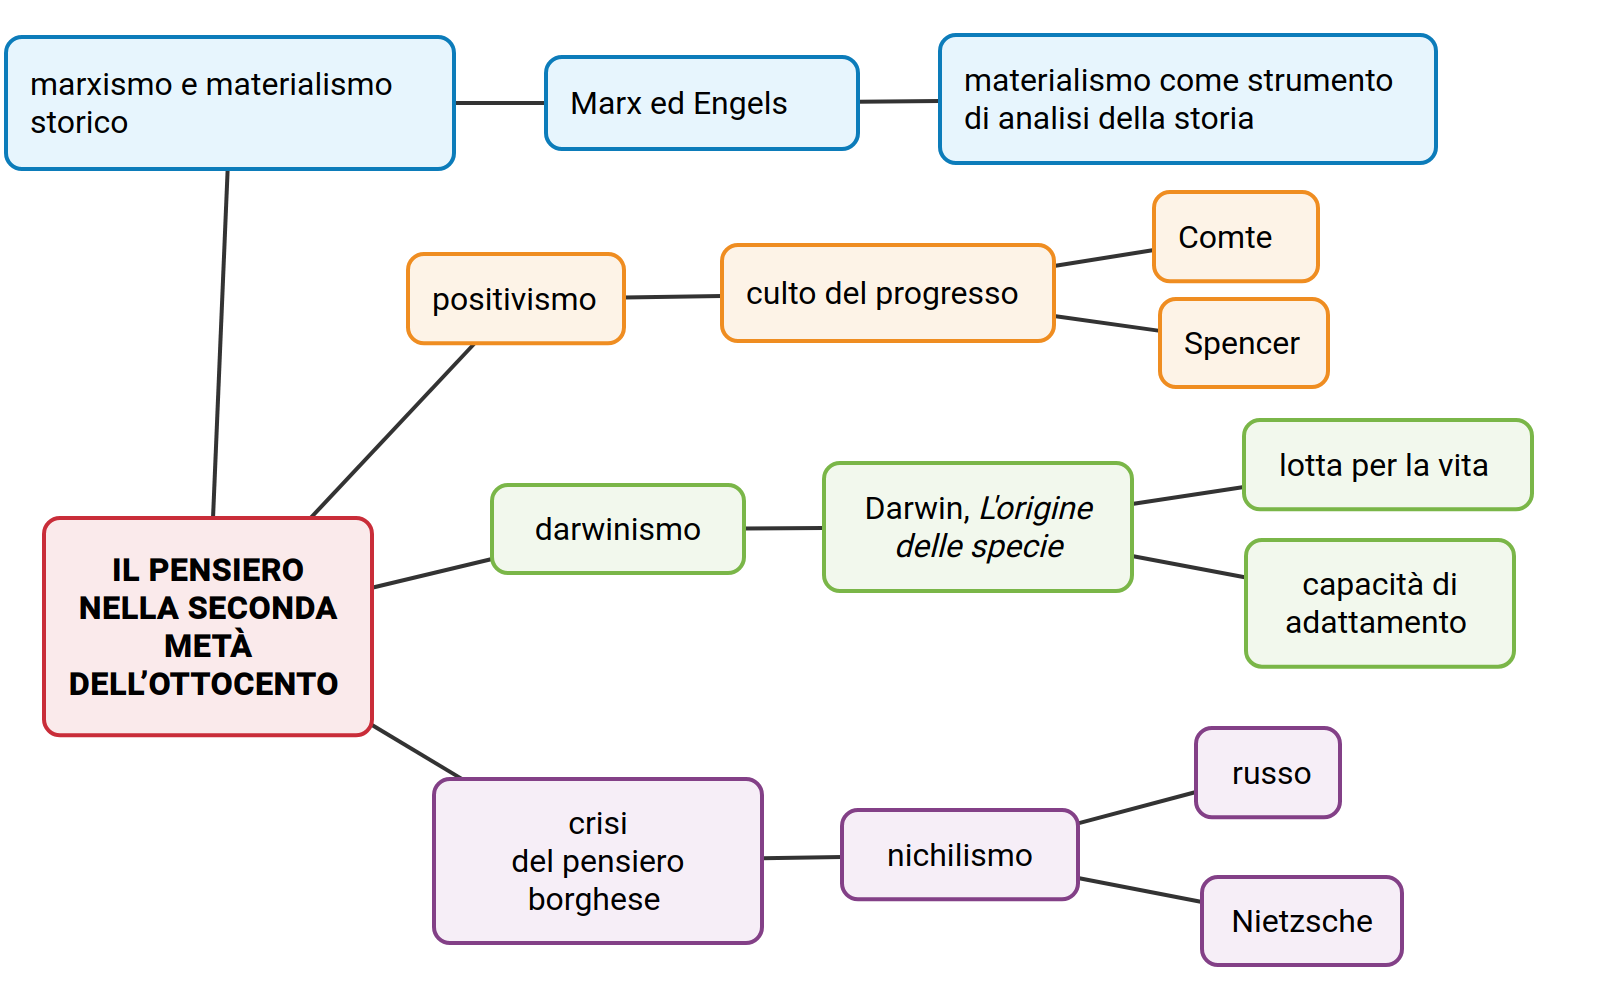
\includegraphics[width=0.75\textwidth]{./graphs/map-situazione2o800.png}

\section{L'età del realismo}
\\
\subsubsection{L’Occidente va veloce}
\\
Nel secondo Ottocento, il ritmo accelerato dei cambiamenti richiede un'attenzione particolare quando si esamina la letteratura di questo periodo. Storicamente, il Regno Unito e la Francia continuano a costruire grandi imperi coloniali, mentre la borghesia del mondo degli affari e del commercio, come descritta nei romanzi di Balzac, rafforza il proprio potere. Le due "nazioni in ritardo", Germania e Italia, raggiungono finalmente l'unità politica.
\\
\\
\nt{Honoré de Balzac, uno dei principali scrittori francesi del XIX secolo, è celebre per la sua monumentale serie di romanzi intitolata "La Commedia Umana". Nato nel 1799 a Tours, in Francia, Balzac si è dedicato a ritrarre la società e la cultura della sua epoca attraverso una vasta panoramica di personaggi e ambientazioni.
\\
\\
La "Commedia Umana" comprende più di 90 romanzi e racconti, con l'obiettivo di offrire una rappresentazione completa della società francese. Le opere sono suddivise in diversi cicli, ciascuno focalizzato su aspetti specifici della vita, dalla vita parigina all'ambiente provinciale, dall'alta società ai ceti più umili.
\\
\\
Balzac è noto per il suo stile realistico e dettagliato, caratterizzato da una descrizione minuziosa dei personaggi e dell'ambiente circostante. Tra le opere più celebri ci sono "Il padre Goriot", che esplora i temi della cupidigia e dell'ambizione sociale, e "Lost Illusions", un'analisi critica del mondo della stampa e delle illusioni perdute nella ricerca del successo.
\\
\\
Il suo contributo al genere del romanzo realista ha influenzato molti scrittori successivi e ha fornito una preziosa testimonianza della vita e della cultura del suo tempo. La figura di Balzac è spesso associata alla dedizione al lavoro e all'ambizione creativa, riflettendo la sua stessa intensa dedizione alla scrittura.}
\\
\\
\subsubsection{Gli  studenti  e  i  critici  della  società}
\\
Nella storia delle idee, si assiste alla chiusura della stagione dell'idealismo tedesco e dei grandi sistemi filosofici. I pensatori più interessanti si presentano soprattutto come critici della società. Dopo la pubblicazione del Manifesto del Partito Comunista nel 1848 insieme a Friedrich Engels, Karl Marx sviluppa la sua rivoluzionaria teoria economica in "Il Capitale" nel 1867. Contemporaneamente, il filosofo tedesco Friedrich Nietzsche, attraverso saggi e libri di aforismi, elabora una critica della vita moderna e delle idee che la guidano, comprese quelle del cristianesimo, dell'etica borghese e della filosofia occidentale.
\\
\subsubsection{La  fiducia  nella  scienza}
\\
La pubblicazione de "L'origine delle specie" di Charles Darwin nel 1859 rivoluziona la concezione dell'uomo, che viene declassato da signore della natura a una fra le tante specie animali sulla Terra, in particolare, una scimmia sapiente. Questo cambiamento profondo nella visione del mondo consolida la fiducia nel metodo scientifico. La scienza e la tecnica dimostrano la loro capacità di modificare e migliorare il mondo: le distanze si accorciano grazie all'ampliamento della rete ferroviaria e all'estensione della rete del telegrafo, malattie considerate incurabili vengono debellate, e il miglioramento delle tecniche di stampa facilita la diffusione di libri e giornali.
\\
\subsubsection{Come cambia il romanzo di formazione}
\\
Nel romanzo del secondo Ottocento, l'influenza dei fatti e delle idee emergenti si riflette chiaramente nei generi e nei temi trattati. Il romanzo di formazione, nato con "Gli anni di apprendistato di Wilhelm Meister" di Goethe e arricchito da autori come Jane Austen, Charles Dickens e Stendhal nella prima metà dell'Ottocento, giunge a una fase di conclusione e trasformazione. In questo contesto, "Enrico il verde" (1855) di Gottfried Keller si colloca nel solco del Wilhelm Meister di Goethe, mentre "L'educazione sentimentale" (1869) di Gustave Flaubert, pur presentandosi come una storia di educazione, narrando di una mancata integrazione, rappresenta un'educazione fallita. A differenza dei giovani pieni di speranza dei romanzi del primo Ottocento, come il Rastignac di Balzac o il Renzo di Manzoni, i protagonisti di questo periodo non riescono a trovare un posto nella società. Al contrario, vivono in conflitto con il mondo e alla fine soccombono, ritirandosi.
\\
\\
\nt{Johann Wolfgang von Goethe (1749-1832) è stato uno dei più importanti scrittori e pensatori tedeschi del periodo classico. La sua opera più celebre è il romanzo epistolare "I dolori del giovane Werther", che ottenne un notevole successo. Goethe ha anche scritto il dramma "Faust", un capolavoro che esplora temi filosofici e morali.
\\
\\
Oltre alla sua produzione letteraria, Goethe ha svolto un ruolo rilevante nella scienza, in particolare con la teoria dei colori. Ha ricoperto varie cariche pubbliche e ha avuto una vita molto poliedrica, esplorando diversi campi artistici e scientifici. La sua influenza si estende oltre i confini tedeschi, contribuendo in modo significativo al Romanticismo europeo.}
\\
\nt{Jane Austen (1775-1817) è stata una famosa scrittrice inglese, nota per i suoi romanzi ironici e satirici che ritraggono la società e le convenzioni del suo tempo. Le sue opere più conosciute includono "Orgoglio e pregiudizio", "Emma" e "Ragione e sentimento". Austen ha enfatizzato il ritratto realistico dei personaggi e ha spesso esplorato temi legati al matrimonio e alle dinamiche sociali.
\\
\\
Nonostante la sua modesta cerchia di lettori durante la sua vita, il lavoro di Jane Austen ha guadagnato popolarità nel corso del tempo, diventando una figura di spicco nella letteratura inglese. La sua abilità nell'analisi psicologica e nell'umorismo ha contribuito a renderla un'autrice amata e studiata ancora oggi.}
\\
\nt{Charles Dickens (1812-1870) è stato uno dei più famosi scrittori vittoriani, noto per i suoi romanzi che ritraggono vividamente la vita sociale dell'Inghilterra del XIX secolo. Opere celebri includono "David Copperfield", "Grandi speranze" e "Canto di Natale". Dickens ha spesso denunciato le ingiustizie sociali e la povertà attraverso i suoi personaggi memorabili e il suo stile narrativo coinvolgente.
\\
\\
Il suo contributo alla letteratura include anche la creazione di personaggi indimenticabili come Scrooge e Oliver Twist. Dickens ha lasciato un'impronta duratura, influenzando la narrativa realista e la coscienza sociale nella letteratura inglese.
}
\\
\nt{Stendhal, pseudonimo di Marie-Henri Beyle (1783-1842), è stato uno scrittore francese noto per i suoi romanzi realisti e psicologici. La sua opera più celebre è "Il rosso e il nero", che esplora la società postnapoleonica attraverso la storia di Julien Sorel, un giovane ambizioso. Stendhal era interessato alla psicologia dei personaggi e alle dinamiche sociali, influenzando il realismo letterario successivo. La sua scrittura si distingue per uno stile analitico e per la profondità psicologica nei ritratti dei protagonisti. La sua influenza si estende oltre la sua epoca, contribuendo alla formazione della narrativa moderna.
}
\\
\nt{Gottfried Keller (1819-1890) è stato uno scrittore svizzero noto per il suo contributo alla letteratura realista del XIX secolo. Tra le sue opere più famose c'è il romanzo "Gli zingari" (Die Leute von Seldwyla), una raccolta di novelle che esplorano la vita e la cultura della Svizzera. Keller ha sperimentato con vari generi letterari, includendo anche poesie e saggi. Il suo stile è caratterizzato da una rappresentazione accurata della vita quotidiana e da una profonda comprensione della psicologia umana. La sua influenza sulla letteratura svizzera e tedesca è riconosciuta come significativa.
}
\\
\\
\subsubsection{Il romanzo storico}
\\
Nella seconda metà dell'Ottocento, il romanzo storico persiste come genere significativo, con opere come "Guerra e pace" di Tolstòj e "Salammbô" di Flaubert. Contestualmente, i romanzi competono con gli studi sociali, focalizzandosi sull'analisi dei costumi e dei modi di vita, specialmente delle classi più umili. Scrittori come i fratelli de Goncourt e Émile Zola, attraverso opere come il ciclo dei Rougon-Macquart, dipingono ritratti intensamente realistici della società francese del XIX secolo, ispirandosi alla cronaca quotidiana.
\\
\\
\nt{Lev Tolstoj (1828-1910) è stato uno dei più grandi scrittori russi, celebre per i suoi capolavori come "Guerra e pace" e "Anna Karenina". Tolstoj ha scritto romanzi epici che esplorano profondamente la psicologia dei personaggi e le dinamiche sociali della Russia dell'epoca. Oltre alla sua produzione letteraria, Tolstoj ha sviluppato idee filosofiche e spirituali, abbracciando il cristianesimo non ortodosso e proponendo concetti di non-violenza e resistenza passiva. La sua eredità letteraria e filosofica continua a esercitare un'influenza duratura nella letteratura mondiale.}
\\
\nt{I fratelli Edmond (1822-1896) e Jules (1830-1870) de Goncourt sono stati due scrittori e critici letterari francesi, noti soprattutto per aver vinto congiuntamente il premio Goncourt, istituito in loro onore. La loro collaborazione ha prodotto opere innovative, come il romanzo "Germinie Lacerteux," che ha affrontato temi sociali e psicologici in modo realistico. I de Goncourt sono considerati precursori del naturalismo e hanno giocato un ruolo significativo nell'evoluzione della letteratura francese del XIX secolo. Jules de Goncourt morì prematuramente nel 1870, ma Edmond ha continuato a sostenere l'eredità letteraria della coppia.
}
\\
\\
\subsubsection{Il  romanzo  e  l’analisi  psicologica  dei  personaggi}
\\
Nei romanzi del secondo Ottocento, emerge una profonda vocazione al realismo, ma ciò che li rende straordinariamente avvincenti è la capacità di penetrare psicologicamente nei personaggi. Scrittori come Dostoevskij ed Eliot dimostrano un'analisi e descrizione sempre più approfondite della vita interiore dei loro personaggi. Questi romanzieri anticipano, secondo Sigmund Freud, molte scoperte sull'inconscio, rendendo il romanzo uno strumento non solo per indagare la realtà oggettiva ma anche per esplorare ciò che accade nei mondi interiori dei personaggi. Nei romanzi degli ultimi decenni del secolo, come quelli di Stevenson, James e Conrad, i personaggi e le loro passioni prendono sempre più il centro della scena, relegando lo sfondo storico in secondo piano.
\\
\nt{Sigmund Freud è stato un pioniere della psicoanalisi, una disciplina che ha rivoluzionato la comprensione della mente umana. Nato nel 1856 a Freiberg, nell'Impero Austro-Ungarico, Freud sviluppò teorie che influenzarono la psicologia, la psichiatria e la cultura in generale. La sua concezione dell'inconscio come motore di comportamenti e desideri, la struttura della personalità divisa tra l'io, l'Es e il Super-Io, e la teoria del complesso edipico sono tra i suoi contributi più significativi.
\\
\\
Freud introdusse il concetto di "libido" come energia psichica, e la sua pratica terapeutica si basava sulla psicoanalisi, un metodo per esplorare l'inconscio attraverso l'analisi dei sogni e l'associazione libera. Tra le sue opere più influenti vi sono "L'interpretazione dei sogni" e "Tre saggi sulla teoria della sessualità". Nonostante le critiche e il dibattito che le sue teorie hanno generato, Freud ha lasciato un'impronta indelebile nella comprensione della mente e del comportamento umano. La psicoanalisi ha influenzato diverse discipline, dall'arte alla letteratura, contribuendo a plasmare il pensiero del XX secolo. Freud è morto a Londra nel 1939.
}
\\
\\
\subsubsection{Una geografia del romanzo}
\\
Nella seconda metà dell'Ottocento, la Francia e il Regno Unito continuano a essere prolifici nella produzione di capolavori narrativi, affiancate ora dalla Russia con autori come Dostoevskij, Tolstòj, Čechov e Turgenev. Tuttavia, la novità più significativa proviene dagli Stati Uniti, dove sta emergendo una tradizione narrativa nazionale. Edgar Allan Poe, uno scrittore statunitense della prima metà del secolo, già aveva influito in Europa con i suoi racconti misteriosi, contribuendo anche alla nascita del romanzo poliziesco. La metà del secolo vede un'esplosione della letteratura americana con opere come "La lettera scarlatta" di Nathaniel Hawthorne nel 1850, "La capanna dello zio Tom" di Harriet Beecher Stowe nel 1852 e "Walden" di Henry David Thoreau nel 1854, un libro simbolo del movimento ambientalista. Nel 1851 esce anche "Moby Dick" di Herman Melville, considerato un capolavoro della letteratura moderna.
\\
\nt{Edgar Allan Poe, nato nel 1809, è stato un autore e poeta americano noto per i suoi racconti gotici e le poesie macabre. La sua vita è stata segnata da tragedie, e questo si riflette nelle sue opere, intrise di oscurità e mistero. Poe è celebre per il suo stile distintivo e la maestria nel creare atmosfere suggestive e inquietanti.
\\
\\
Tra le sue opere più famose vi sono "Il corvo", una poesia emblematica del suo stile, e racconti come "L'orrore di Red Hook" e "La caduta della casa degli Usher". La sua influenza si estende alla letteratura gotica e al genere del giallo, contribuendo a plasmare la narrativa dell'orrore. Poe morì nel 1849 a Baltimora, lasciando un'impronta duratura sulla letteratura americana.}
\\
\\
\subsubsection{Il romanzo in Italia}
\\
Nell'Italia della seconda metà dell'Ottocento, dopo il successo dei "Promessi Sposi" nella prima metà del secolo, il romanzo attraversa un periodo di crisi e non emerge alcun autore italiano equiparabile a Flaubert, Tolstòj o Dostoevskij. Tuttavia, vi sono alcuni romanzi italiani che meritano di essere considerati parte della grande letteratura mondiale. Nonostante la continuazione della moda del romanzo storico, con una correzione rispetto a Manzoni, che si sposta verso i primi anni dell'Ottocento o gli anni del Risorgimento, alcuni romanzi italiani spiccano per appartenere a tendenze e generi diversi, testimoniando una tradizione vitale e multiforme.
\\
\\
Giovanni Verga, uno dei maggiori scrittori italiani del periodo, focalizza la sua attenzione sulla società siciliana contemporanea nei capolavori "I Malavoglia" (1881) e "Mastro-don Gesualdo" (1889). Verso la fine del secolo, altri due grandi scrittori italiani, Gabriele d'Annunzio nel 1889 con "Il piacere" e Italo Svevo nel 1892 e 1898 con "Una vita" e "Senilità", si concentrano più sulla psiche dei loro personaggi che sui meccanismi sociali, mostrando tracce della loro stessa personalità nei protagonisti.
\\
\section{Gustave Flaubert}
\\
\subsubsection{Una  vita  tranquilla  tra  Parigi  e  la  Normandia}
\\
Gustave Flaubert, il più importante romanziere francese dell'Ottocento, nacque il 12 dicembre 1821 a Rouen, in Normandia. Sin da giovane si interessò alla letteratura, scrivendo le sue prime prove narrative come "Memorie di un folle" (1838) e "Novembre" (1842). Dopo il liceo, si trasferì a Parigi per studiare legge, ma presto abbandonò gli studi per dedicarsi interamente alla letteratura. Nel 1846, a causa di una malattia nervosa, interruppe gli studi e si ritirò a Croisset, in Normandia, dove trascorse il resto della sua vita. Nel corso degli anni, fece un lungo viaggio in Medio Oriente e in Italia (1849-1851). La sua opera più nota, "Madame Bovary," fu pubblicata nel 1857 e la sua attenzione alla precisione stilistica e alla profondità psicologica ebbe un'influenza duratura su generazioni di scrittori successivi.
\\
\subsubsection{I  romanzi  e  le  ultime  opere}
\\
Dopo il viaggio in Oriente, Flaubert inizia a lavorare su "Madame Bovary," che pubblica nel 1856 con grande successo e scandalo. Nel 1862, esce "Salammbô," un romanzo storico ambientato a Cartagine. Nel 1869, completa "L'educazione sentimentale," che riceve scarso successo. Nel 1877, i suoi "Tre racconti" sono ben accolti. Flaubert inizia la stesura di "Bouvard e Pécuchet," un romanzo satirico sulla stupidità umana, ma muore nel maggio del 1880, lasciando l'opera incompiuta. Postumi escono racconti giovanili e l'Epistolario, uno dei più ricchi dell'Ottocento.
\\
\subsubsection{I temi e le idee: dall’eccezione alla norma}
\\
Nell'Ottocento, gli scrittori si allontanano dalle storie di esseri eccezionali e iniziano a raccontare la vita ordinaria delle persone comuni. Flaubert è uno dei protagonisti di questa rivoluzione narrativa.
\\
\subsubsection{Il metodo: dissezionare la realtà}
\\
Flaubert, influenzato dalle osservazioni del padre chirurgo, sviluppa uno sguardo realistico, oggettivo e scrupoloso nella sua scrittura. Le sue esperienze giovanili, come l'osservazione di dissezioni e il confronto con la follia, contribuiscono a formare un talento realistico che caratterizza i suoi romanzi, tra cui "Madame Bovary", "L'educazione sentimentale" e "Bouvard e Pécuchet". La sua capacità di "dissezionare" la realtà, senza tremori emotivi, rende le sue opere straordinariamente interessanti.
\\
"dissezionare la realtà" significa analizzare e descrivere la vita e le esperienze umane con grande dettaglio e precisione. Flaubert era noto per la sua attenzione scrupolosa ai dettagli e alla precisione nella rappresentazione delle situazioni, dei personaggi e degli ambienti nei suoi romanzi. Il termine "dissezionare" richiama l'immagine di un anatomista che esamina con attenzione e in modo scientifico le parti di un corpo. Nel caso di Flaubert, questo approccio si riflette nella sua scrittura realistica e nell'osservazione obiettiva della società, delle relazioni umane e delle condizioni umane, senza sentimentalismi o idealizzazioni. La sua opera è caratterizzata da una rappresentazione accurata e spesso critica della realtà.
\\
\subsubsection{Un’epica borghese}
\\
Flaubert si concentra sulla borghesia francese nei suoi scritti, analizzando non solo la realtà oggettiva esterna, ma soprattutto la mentalità di questa classe sociale. Contrariamente a Balzac, Flaubert non si interessa tanto al modo in cui la borghesia vive o alle sue dinamiche sociali, ma esplora la mentalità borghese modellata da convenzioni che egli guarda con ironia e disprezzo. I suoi nemici principali sono la bestialità, l'idiota, la banalità e i luoghi comuni, che considera i veri protagonisti dei suoi romanzi, come in "Madame Bovary," dove la protagonista viene simbolicamente uccisa dalla mentalità borghese, e in "Bouvard e Pécuchet," una sorta di catalogo delle sciocchezze che riempivano le menti borghesi del suo tempo.
\\
\subsubsection{Madame Bovary}
\\
\subsubsubsection{Il successo e lo scandalo}
\\
"Madame Bovary: Costumi di provincia" fu pubblicato a puntate nel 1856 sulla "Revue de Paris" e l'anno successivo in volume. Il romanzo ottenne un grande successo e provocò un notevole scandalo. Flaubert fu citato in giudizio per aver offeso la morale e la religione, ma alla fine del processo, sostenuto da eminenti scrittori dell'epoca come Charles Baudelaire e Charles-Augustin de Sainte-Beuve, fu assolto.
\\
\subsubsection{Emma: tra la monotona provincia e il sogno aristocratico}
\\
Madame Bovary, nota anche come Emma, è un'orfana educata in modo sommario in un collegio di suore. Dopo aver sposato Charles Bovary, un modesto medico di provincia, la coppia conduce una vita monotona a Tostes. Tutto cambia quando Emma, desiderosa di appartenere al mondo aristocratico, partecipa a un ballo, dopo il quale non riesce più ad adattarsi alla vita grigia della provincia.
\\
\subsubsection{Delusione,  crisi  e  suicidio}
\\
Dopo aver avuto una figlia, Berthe, Emma Bovary non trova appagamento nella maternità. Si innamora di Léon, un giovane praticante di un notaio, ma lui la lascia per studiare Legge a Parigi. Successivamente, Emma ha una breve relazione con Rodolphe, un uomo senza scrupoli che la abbandona. Per consolarsi, riprende il rapporto con Léon. Le sue infedeltà diventano di dominio pubblico, e per finanziare la sua vita costosa, contrae un grande debito con uno strozzino. Minacciata di denuncia, chiede aiuto a Rodolphe, ma quest'ultimo rifiuta. Disperata, Emma si suicida ingerendo dell'arsenico.
\\
\newpage
\\
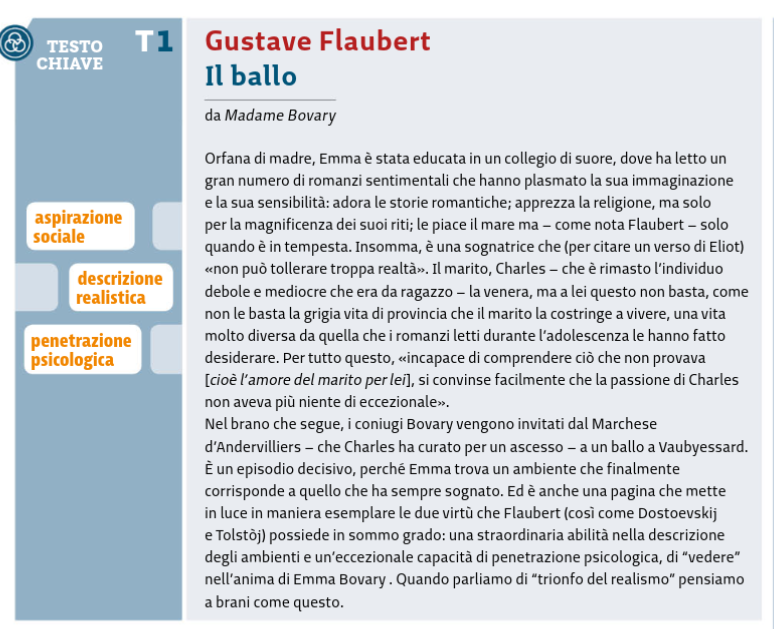
\includegraphics[width=0.75\textwidth]{./graphs/gustave-flaubert-il-ballo.png}
\\
In questo brano, Flaubert utilizza la prospettiva di Emma per descrivere il suo ingresso nel mondo aristocratico e il suo senso di inadeguatezza. Gli invitati, un domestico, una signora, un ballerino, sono descritti in modo generico, senza nomi, poiché compaiono e scompaiono rapidamente, come sfocati sullo sfondo. La scena è vista attraverso gli occhi confusi di Emma, che partecipa per la prima volta a un ballo di gala.
\\
\\
Flaubert crea un senso di euforia nel lettore, poiché tutto ciò che Emma vede è nuovo e inaspettato. Tuttavia, questo senso di appartenenza è effimero. Emma si rende conto della sua estraneità a questo mondo aristocratico e Flaubert enfatizza la sua consapevolezza di non appartenere a quel contesto.
\\
\\
La geniale invenzione di Flaubert si manifesta quando Emma, dalla finestra, vede dei contadini che osservano gli invitati. Questo momento sottolinea la differenza tra la sua vita attuale e le sue radici contadine. Flaubert evita di esplicitare il pensiero di Emma, ma emerge chiaramente il contrasto tra la giovinezza in campagna e la situazione attuale, tra la memoria della fattoria e il lusso della festa.
\\
\\
Inoltre, Flaubert utilizza pochi tratti descrittivi per evidenziare la differenza sociale di Emma. Charles, suo marito, appare sonnecchiante durante la festa, incapace di apprezzare il lusso. La sua reazione ai giochi e la soddisfazione nel togliersi gli stivali simboleggiano la sua estraneità al mondo aristocratico.
\\
\\
Infine, il destino di Emma viene implicitamente suggerito quando, alla fine della festa, si domanda se questo sarà il suo destino. La risposta sarà il suo rifiuto di accettare quella vita, conducendola alla tragica scelta del suicidio. Flaubert si distingue nella sua capacità di far emergere i pensieri dei personaggi attraverso le azioni descritte, senza bisogno di esprimerli esplicitamente.
\\
\newpage
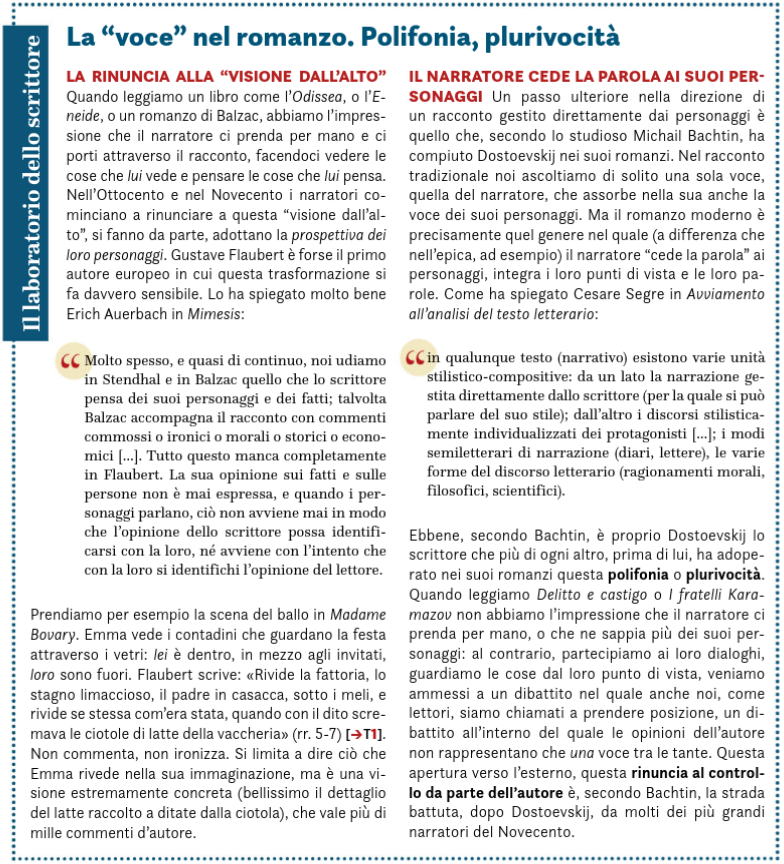
\includegraphics[width=0.90\textwidth]{./graphs/la-voce-nel-romanzo.png}
\newpage
\section{Le radici culturali del Verismo}
\subsubsection{Rappresentare  la  realtà  in  pittura,  a  teatro}
\\
Nel panorama culturale del secondo Ottocento, molti artisti e intellettuali, inclusi pittori, scultori, fotografi, filosofi e letterati, sembrano dedicarsi a rappresentare con precisione, originalità e profondità la realtà o almeno un suo frammento. Nella pittura, ispirati dal realismo di artisti come Daumier, Courbet e Millet, i macchiaioli italiani abbandonano l'idealismo e si impegnano a osservare e ritrarre la realtà con scrupolo realistico. Nel teatro, si afferma il dramma borghese, con autori che cercano di portare in scena fatti e personaggi appartenenti al mondo borghese degli spettatori. Sebbene l'Italia non abbia autori paragonabili a Cechov o Ibsen, si percepisce una svolta realistica anche nei teatri italiani, con Luigi Capuana come teorico del Verismo, notevole critico teatrale e scrittore.
\\
\\
\nt{Honoré Daumier, vissuto nel XIX secolo, è stato un acclamato pittore, scultore e caricaturista francese. La sua opera è caratterizzata da una critica sociale penetrante e satirica nei confronti delle élite borghesi e politiche della sua epoca. Daumier ha utilizzato la sua abilità artistica per rappresentare la complessità della vita quotidiana, evidenziando le ingiustizie sociali e le contraddizioni della società francese dell'Ottocento.
\\
\\
La sua visione artistica è particolarmente evidente nelle sue celebri caricature, che ritraggono vividamente la corruzione, l'ipocrisia e la disuguaglianza. Daumier è stato un osservatore acuto della realtà e ha influenzato significativamente il realismo artistico. La sua eredità artistica è ancora riconosciuta come un potente strumento di critica sociale.}
\\
\nt{Gustave Courbet, figura centrale del movimento realista del XIX secolo, fu un pittore francese noto per la sua rappresentazione sincera e diretta della vita quotidiana. Courbet si distinse per il suo rifiuto delle convenzioni artistiche dell'epoca e per la sua enfasi sulla rappresentazione onesta della realtà. La sua visione artistica era caratterizzata da un atteggiamento anti-romantico e anti-idealista, puntando a una pittura più aderente alla vita reale.
\\
\\
Courbet credeva nell'arte come strumento per riflettere la vera natura dell'esistenza umana, sfidando l'estetica idealizzata prevalente nel periodo romantico. La sua famosa opera "L'Origine du monde" è emblematica della sua audacia nel trattare tematiche considerate tabù. Courbet ha contribuito significativamente a ridefinire il ruolo dell'artista e dell'arte nella società dell'Ottocento.}
\\
\nt{Jean-François Millet, pittore francese del XIX secolo, fu una figura chiave del movimento realista. Millet divenne famoso per le sue rappresentazioni della vita contadina, enfatizzando la dignità del lavoro agricolo. La sua visione artistica era caratterizzata da un forte impegno sociale, ritraendo le condizioni reali dei contadini e degli agricoltori.
\\
\\
Millet rifiutava l'idealizzazione romantica della campagna e si concentrava sulla rappresentazione autentica della fatica e della semplicità della vita rurale. La sua opera più celebre, "L'Angélus," incarna il suo interesse per il lavoro umile e la spiritualità. Millet, attraverso la sua pittura realista, ha contribuito a sensibilizzare il pubblico sulle sfide e le realtà della vita quotidiana dei contadini, sottolineando il valore della classe lavoratrice nella società.
}
\\
\nt{Luigi Capuana è stato uno scrittore e critico letterario italiano, nato nel 1839 e morto nel 1915. È stato una figura di spicco nel movimento verista italiano, insieme a Giovanni Verga. Capuana contribuì a definire e promuovere il realismo letterario in Italia.
\\
\\
La sua opera più nota è "Il Marchese di Roccaverdina," un romanzo verista che esplora le dinamiche sociali e morali della Sicilia dell'epoca. Capuana fu anche coinvolto nell'ambiente culturale e letterario, fondando la rivista "La Cronaca Bizantina" e partecipando alla vita intellettuale del suo tempo.
\\
\\
Come critico letterario, Capuana fu uno dei primi a introdurre in Italia le teorie naturaliste di Émile Zola. La sua attività critica ebbe un impatto significativo sulla percezione e sulla produzione letteraria in Italia, contribuendo alla formazione di nuove correnti e stili letterari.
}
\\
\\
\subsubsection{La filosofia: il Positivismo}
\\
Il Positivismo, che caratterizza la filosofia del secondo Ottocento, ha come principale esponente Auguste Comte. Questa corrente sostiene che il progresso umano è legato alla scoperta di leggi universali che governano diversi ambiti della vita, dalla fisica all'etica. Comte, uno scienziato sociale, ha influenzato l'Europa, specialmente attraverso il lavoro del suo discepolo Hippolyte Taine, che ha sviluppato e semplificato la visione positivista in chiave deterministica, enfatizzando razza, ambiente e momento come fattori chiave.
\\
\\
\nt{Hippolyte Taine (1828-1893) è stato un influente filosofo e critico letterario francese del XIX secolo, noto per il suo approccio positivista alla critica. La sua opera principale, "La Filosofia dell'Arte," applica il metodo scientifico all'analisi delle opere d'arte, cercando di identificare i fattori influenti. Taine introdusse il concetto di "determinismo" sostenendo che l'ambiente fisico, sociale e razziale determina la natura individuale e sociale. Questa idea ha influenzato il naturalismo letterario e il determinismo dell'epoca. La sua "Storia della Letteratura Inglese" esamina lo sviluppo letterario inglese sotto vari fattori ambientali e sociali, contribuendo in modo duraturo alla critica letteraria.}
\\
\\
\subsubsection{La letteratura: il Naturalismo}
\\
Nel contesto letterario del secondo Ottocento, Émile Zola, rappresentante principale del Naturalismo, fu fortemente influenzato dalle idee di Auguste Comte e Hippolyte Taine. Zola cercò di creare un "romanzo sperimentale" basato sul metodo scientifico, osservando e descrivendo oggettivamente la realtà contemporanea, con particolare attenzione alle classi emarginate. La sua narrazione era impersonale, riducendo al minimo l'intervento dell'autore. Queste influenze si riflettono anche nelle opere di autori italiani come Verga, Capuana e De Roberto.
\\
\newpage
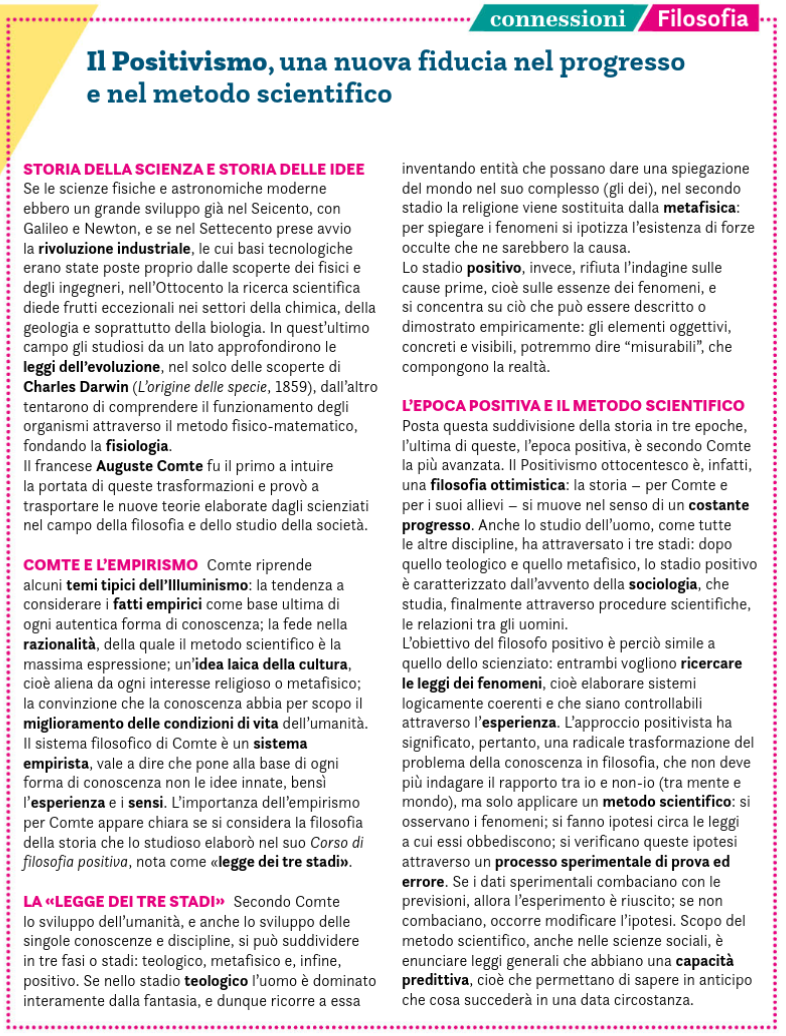
\includegraphics[width=0.90\textwidth]{./graphs/ilpositivismo-fiducia nel progresso.png}
\newpage
\section{Zola e il Naturalismo}
\\

\\
\subsubsection{I  primi  romanzi  naturalisti}
\\
Nel contesto del Naturalismo, i primi romanzi che possono essere considerati pienamente naturalisti includono "Germinie Lacerteux" (1865) dei fratelli Edmond e Jules de Goncourt, che narra la storia di una donna di servizio rovinata dall'amore per un uomo senza scrupoli, e soprattutto "Thérèse Raquin" di Émile Zola (1867). Quest'ultimo racconta la storia di una donna che uccide il marito per poter sposare un altro uomo, Laurent, e entrambi, oppressi dal rimorso, si suicidano. Nella prefazione alla seconda edizione di "Thérèse Raquin", Zola enfatizza il suo interesse nello studio dei "temperamenti" piuttosto che nell'indagine sui "caratteri individuali", sottolineando il determinismo che guida lo sviluppo degli eventi nel romanzo attraverso i temperamenti dei personaggi.
\\
\subsubsection{Zola e la saga dei Rougon-Macquart}
\\
Attratto dalle idee di Auguste Comte sulla sociologia e dalle ricerche di Charles Darwin sulla selezione naturale, Émile Zola nei suoi romanzi presta particolare attenzione all'ambiente sociale dei personaggi. Si focalizza soprattutto sulla vita dei poveri, descrivendo la realtà dagli operai (come in "L’ammazzatoio", 1876) ai lavoratori precari in un grande magazzino ("Il paradiso delle signore", 1883) fino alle prostitute d'alto bordo ("Nanà", 1880). Il risultato è una saga di venti romanzi intitolata "I Rougon-Macquart", che offre un affresco della società francese dell'Ottocento, concentrandosi sulle vicende della famiglia Rougon-Macquart.
\\
\subsubsection{Lo scrittore come lo scienziato}
\\
Nel saggio del 1880 intitolato "Il romanzo sperimentale", Zola spiega il suo progetto affermando che, poiché la medicina è passata da un'arte a una scienza grazie al metodo sperimentale, anche la letteratura potrebbe diventare una scienza usando lo stesso approccio. L'arte, secondo Zola, dovrebbe riprodurre la realtà e identificare le cause dei comportamenti umani e le leggi che li governano. Immagina lo scrittore come uno scienziato in camice bianco che lavora sui suoi personaggi come farebbe uno scienziato con le cavie da laboratorio. Il sottotitolo della sua saga "I Rougon-Macquart" è "Storia naturale e sociale di una famiglia nel Secondo Impero".
\\
\subsubsection{Zola, scrittore politicamente impegnato}
\\
Zola non concepisce un'arte asettica; al contrario, si considera uno scrittore politicamente impegnato. Desidera che i suoi libri non siano semplici mezzi di intrattenimento, ma che invece aprano gli occhi del pubblico facendolo riflettere sulla miseria e disumanità in cui milioni di persone vivono nelle grandi città industriali come Parigi.
\\
\subsubsection{Milieu, moment, race e determinismo}
\\
La figura di Gervaise, protagonista del romanzo "L'ammazzatoio" (o "L'assomoir"), rappresenta un esempio emblematico della concezione zoliana. A causa della miseria del suo quartiere operaio, dei suoi difetti fisici e del contesto storico del Secondo Impero, a Gervaise è preclusa ogni possibilità di ascesa sociale. L'ambiente, il momento storico e la razza concorrono nel determinare il suo destino tragico.
\\
\subsubsection{La voce del narratore: determinismo e denuncia}
\\
I caratteri principali dello scrittore naturalista, secondo Zola, includono il determinismo, in cui ambiente, razza e momento storico influenzano il destino degli individui; l'uso del metodo sperimentale, dove i personaggi agiscono in situazioni tipiche; l'impersonalità del narratore che si focalizza sugli aspetti esteriori; e l'impegno sociale, cercando di sensibilizzare il pubblico sulle condizioni di vita della classe operaia attraverso documentazione accurata.
\\
\subsubsection{Il romanzo sperimentale}
\\
Zola fu accusato di immoralità, oscenità e gusto per il triviale a causa delle sue storie su prostitute, alcolizzati e piccoli criminali, suscitando disgusto nel pubblico borghese conservatore. Rispose alle accuse in vari scritti teorici e nella raccolta di saggi "Il romanzo sperimentale" (1880), difendendo la sua pratica artistica e l'approccio scientifico alla rappresentazione della realtà.
\\
\newpage 
\\
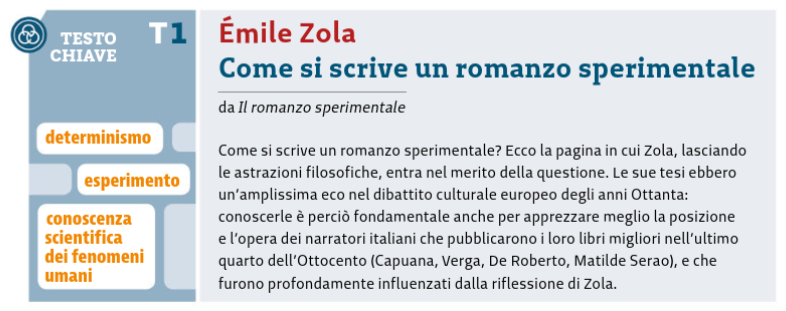
\includegraphics[width=0.90\textwidth]{./graphs/come-si-scrive-un-romanzo-sperimentale.png}
\\
L'analisi di questo brano di Zola evidenzia il suo approccio distintivo al romanzo naturalista, in cui cerca di conciliare la creazione artistica con la rigorosa osservazione scientifica. Zola riconosce la differenza fondamentale tra la letteratura e le scienze fisiche, sottolineando che il romanziere non può semplicemente "osservare" come un fisico o un fisiologo, ma deve essere il creatore attivo della storia.
\\
\\
Per superare questa differenza, Zola invoca le "leggi della natura" a cui il naturalista deve conformarsi. Queste leggi riguardano i comportamenti umani considerati normali in un ambiente e in un'epoca specifici. Inoltre, Zola enfatizza che lo scrittore ha la responsabilità di ideare una trama che metta in evidenza queste leggi della natura attraverso le prove e gli ambienti attraverso i quali fa passare i personaggi.
\\
\\
La concezione di Zola del romanzo sperimentale si basa sulla nozione che i personaggi dei suoi romanzi fungano da rappresentanti sperimentali, campioni di ogni essere umano nelle stesse condizioni. Analogamente al positivismo scientifico, Zola crede che attraverso il metodo osservativo ed esperimentale nel romanzo, si possa comprendere la realtà umana. Pertanto, nel romanzo sperimentale, non c'è solo osservazione, ma anche esperimento, dove i personaggi vengono posti in situazioni specifiche per evidenziare il funzionamento delle loro emozioni, idee e azioni.
\\

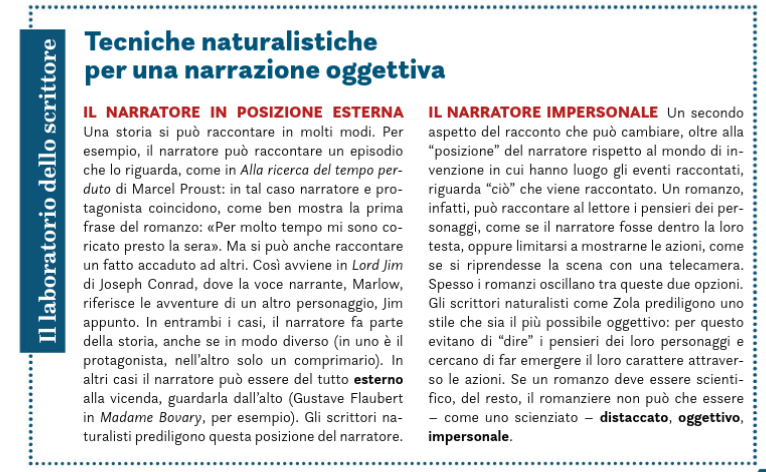
\includegraphics[width=0.90\textwidth]{./graphs/tecnichenarroggettive.png}
\\
\newpage
\\
\subsubsection{Emile zola "Come funziona un romanzo naturalista"}
\\
\\
\subsubsection{Analisi del testo}
\\
Nel racconto di Zola su Gervaise, l'autore adotta una narrativa impersonale tipica del Naturalismo, registrando oggettivamente azioni e parole dei personaggi senza intervenire con giudizi diretti. Tuttavia, Zola occasionalmente permette ai lettori di accedere ai pensieri dei personaggi, mantenendo comunque una certa distanza. Le descrizioni, ricche nei romanzi naturalisti, rafforzano l'impressione di oggettività, come nella rappresentazione della miseria degli operai a Parigi. Zola, sebbene eviti di esprimere giudizi diretti, guida l'interpretazione del lettore, suggerendo le conclusioni sull'antitesi tra ricchi e poveri a Parigi e sul destino tragico dei personaggi. La storia di Gervaise, segnata dalla miseria e dalla tragedia, esemplifica la visione negativa della società parigina del Secondo Impero.
\\
\section{Dal naturalismo al verismo}  
\subsubsection{L’arrivo del romanzo francese in Italia}
\\
Negli anni Settanta, i romanzi naturalisti di Goncourt e Zola entrano nel dibattito letterario italiano. Luigi Capuana elogia "L’ammazzatoio" di Zola nel "Corriere della Sera" (marzo 1877) e pubblica un profilo dello scrittore francese l'anno successivo. Parallelamente, Francesco De Sanctis, eminente critico italiano, dedica articoli al romanzo realista e al Naturalismo francese, successivamente raccolti nello "Studio sopra Emilio Zola" nel 1879.
\\
\subsubsection{La tendenza verista in Italia}
\\
La conoscenza della nuova letteratura francese spinge gli scrittori italiani, già orientati al realismo dalla Scapigliatura, verso la tendenza verista. Nel 1878, Verga pubblica la novella "Rosso Malpelo," seguito nel 1879 da Capuana con il romanzo "Giacinta." Questi lavori, insieme ai successivi di Verga come "I Malavoglia" e le "Novelle rusticane," influenzano numerosi scrittori negli anni Ottanta. Il Verismo si distingue per la documentazione accurata della vita quotidiana, specialmente delle classi inferiori meridionali, accompagnato da una riflessione teorica sulla narrazione. Verga e Capuana sono consapevoli della rivoluzione letteraria in corso, espressa nelle loro opere e scritti teorici.
\\
\subsubsection{La  lezione  di  Zola}
\\
I veristi italiani, fortemente influenzati da Zola, assimilano diverse tecniche, tra cui l'impersonalità del narratore, lunghe descrizioni oggettive e trame semplici. Seguono l'attenzione di Zola all'ambiente sociale, focalizzandosi spesso sui poveri e scegliendo protagonisti umili in situazioni di difficoltà, come i Malavoglia di Verga, una famiglia di pescatori siciliani.
\\
\subsubsection{L’artificio della regressione}
\\
I veristi si discostano dalla poetica naturalista in diversi modi. Dal punto di vista formale, spingono l'impersonalità al punto di affermare che l'autore non deve comparire nel racconto né esprimere i suoi pensieri e giudizi. Adoptano l'"artificio della regressione", col narratore che si pone sullo stesso piano culturale dei personaggi, rinunciando alla prospettiva borghese. Tuttavia, la differenza principale è ideologica: mentre Zola vede l'arte come un mezzo di intervento sociale e di denuncia, Capuana e Verga sottolineano l'autonomia dell'arte, giudicata per il suo valore intrinseco anziché per gli effetti sulla società.
\\
\subsubsection{La società è immutabile}
\\
I naturalisti e i veristi concordano sull'importanza dell'ambiente sull'individuo, ma divergono nella prospettiva. Per i naturalisti, le disuguaglianze sociali influenzano l'ambiente, mentre per i veristi, l'ambiente è visto come un dato naturale e immutabile che agisce invariabilmente su ogni generazione. La divergenza non riguarda solo la differenza tra città e campagna, ma rappresenta una visione contrastante della storia umana. Mentre il Naturalismo abbraccia l'idea positivista di progresso continuo, il Verismo sostiene che i rapporti sociali sono immutabili, sfidando la possibilità di cambiamenti significativi attraverso gli sforzi individuali.
\\
\subsubsection{L’astensione dal giudizio}
\\
Nei romanzi veristi, l'assenza di una "voce" riconducibile all'autore e la centralità dei personaggi eliminano la possibilità di un intervento esterno che guidi il giudizio del lettore o lo spinga a riflettere sulle implicazioni politiche o sociali della storia. Questo non impedisce ai veristi di affrontare tematiche politiche, come dimostra l'esempio di "Rosso Malpelo," scritto da Verga durante un dibattito sull'occupazione minorile in Italia. Tuttavia, i veristi sottolineano l'autonomia dell'arte, affermando che il romanzo offre un'immagine oggettiva della realtà senza fornire interpretazioni esplicite, lasciando al lettore il compito di trarre conclusioni. La prospettiva del narratore è parte integrante del sistema rappresentato nell'opera, senza emettere condanne morali esplicite.
\\
\\
\qs{}{Quali sono le differenze tra naturalismo francese e versismo italano?}
\sol{Le diffirenze tra naturalismo e verismo francese sono 6, il naturalismo ha carattere nazionale si sviluppa in tutta la Francia della seconda metà dell'800 mentre il verismo ha carattere regionale, si sviluppa principalmente nelle regioni della sicilia e della calabria. La seconda differenza riguarda invece l'ambiente in cui sono rappresentati i romanzi per quanto riguarda il naturalismo troviamo una realtà tendenzialmente urbana, nel verismo troviamo invece situazioni provinciali e cittadine, una realtà definibile rurale, i personaggi invece nelle opere naturaliste provengono da realtà operaie provenienti quindi dal proletariato urbano, nel verismo invece troviamo personaggi come pescatori, pastori, contadini, personaggi spesso tralasciati ed emarginati dalla realtà urbana, un'altra differenza è la funzione sociale esercitata dall'arte Zola Flaubert denunciano i problemi legati alla forte industrializzazione della Francia dell'epoca. Nel verismo troviamo la denuncia che riguarda la questione meridoniale come il latifondismo, i contrasti tra ceti sociali o l'analfabetismo, insomma tutti quei problemi che affligono il meridione d'Italia. Un altra differenza può essere vista dal lato linguistico I naturalisti francesi utilizzano una lingua mimetica, ovvero copiano la parlata locale nel verismo ciò non accade, questo è dovuto all'obbiettivo del verismo denunciare i problemi sociali, per questo verga mira al grande pubblico. un altra differenza riguarda l'impersonalità del narrattore, potremmo definire il narratore impersonale naturalista a parte auctoris ovvero dalla parta dell'autore mentre il narratore impersonale verista impersonale dalla parte dell'opera.}
\\
\\
\subsubsection{Dopo il Verismo}
\\
Il periodo del Verismo va dalla fine degli anni Settanta alla fine degli anni Ottanta del XIX secolo, con "I Viceré" di De Roberto che segna la chiusura di questa stagione nel 1894. Negli anni Novanta, Capuana si dedica principalmente a romanzi psicologici e racconti per bambini, mentre Verga, dopo "Mastro-don Gesualdo" nel 1889, si orienta verso il teatro. A partire dal 1889, d'Annunzio pubblica "Il piacere," inaugurando una fase in cui gli scrittori italiani preferiranno l'indagine sulla psicologia decadente di individui singoli rispetto al "realismo sociale" di Zola o Verga. Gli scrittori successivi all'Unità seguiranno strade diverse, e Verga e Capuana saranno riscoperti dalla critica più tardi, dagli anni Venti e Trenta del XX secolo, e ancora di più dagli anni Sessanta in avanti.
\\
\section{Giovanni Verga}
\subsection{Le opere}
\\
\subsubsection{Il “momento verghiano”}
\\
Negli anni Ottanta dell'Ottocento si verifica il "momento verghiano" nella letteratura italiana, caratterizzato dalla pubblicazione dei capolavori di Giovanni Verga, tra cui "Vita dei campi," "I Malavoglia," "Novelle rusticane," e "Mastro-don Gesualdo." Verga, pur avendo scritto molto sin dalla giovinezza, si distingue soprattutto in questo periodo in cui decide di raccontare la vita del popolo siciliano utilizzando nuove tecniche narrative ispirate dai grandi romanzieri francesi come Gustave Flaubert, Guy de Maupassant, e soprattutto Émile Zola.
\\
\subsubsection{I primi romanzi}
\\
Giovanni Verga, nei suoi primi romanzi, aspira a innovare la letteratura italiana, seguendo l'esempio di Balzac e Flaubert nella letteratura francese. Tuttavia, egli mostra un desiderio evidente di ottenere anche il successo, cercando di raggiungerlo attraverso l'uso di tinte melodrammatiche e il lirismo nei caratteri, nelle situazioni e nelle passioni, come evidenziato nelle opere giovanili quali "Una peccatrice," "Storia di una capinera," "Eva," e i romanzi milanesi "Tigre reale" ed "Eros."
\\
\subsubsection{Nedda}
\\
In "Nedda," un bozzetto di Verga, l'autore si allontana dai toni realisti che caratterizzeranno i suoi lavori successivi. La storia si svolge nella campagna siciliana e segue la vita di Nedda, una povera raccoglitrice di olive. Il suo fidanzato Janu muore di malaria mentre lavora, lasciandola incinta. Nedda, dopo aver perso anche la madre, si trova sola con un figlio debole che muore poco dopo la nascita. Nonostante l'ambientazione siciliana e la tematica della vita dei meno fortunati, "Nedda" rimane intriso di patetismo romantico, lontano dalla poetica verista dei successivi "Malavoglia" di Verga.
\\
\subsubsection{I racconti veristi}
\\
Dopo il successo di "Nedda" nel 1874, Giovanni Verga lavora a un nuovo bozzetto siciliano, inizialmente intitolato Padron 'Ntoni. Nel 1877, influenzato dalla lettura de "L'ammazzatoio" di Zola, Verga adotta la tecnica narrativa dello scrittore francese. Nei tre anni successivi, scrive racconti che formeranno la sua prima vera raccolta verista, "Vita dei campi" (1880), e rielabora "Padron 'Ntoni" trasformandolo nel nucleo del successivo romanzo "I Malavoglia," che prende il nome dalla famiglia di pescatori protagonista.
\\
\subsubsection{I Malavoglia e il «ciclo dei vinti»}
\\
Nel progetto di Giovanni Verga, "I Malavoglia" (1881) è il primo di cinque romanzi che avrebbero dovuto coprire la vita delle varie classi sociali sotto il titolo complessivo "Marea." La lettera del 1878 a Salvatore Paola Verdura rivela l'idea di una "fantasmagoria della lotta per la vita" che spazia dal cenciaiuolo al ministro e all'artista, rappresentando drammaticamente, ridicolmente o comicamente le diverse fisionomie sociali. Il ciclo immaginato, non completamente realizzato, si chiamava "Marea," sottolineando un destino collettivo che trascendeva i destini individuali. "I Malavoglia" è un esempio iniziale di questa teoria sociale, raffigurando la tragedia di una famiglia di pescatori siciliani colpita dal naufragio di una barca carica di lupini, investimento finanziario del capofamiglia, Padron 'Ntoni.
\\
\subsubsection{Le  novelle  dei  primi  anni  Ottanta}
\\
Nel primo volume del ciclo "Marea," Giovanni Verga pubblicò solo "I Malavoglia" (1881), mentre il secondo volume, "Mastro-don Gesualdo," uscì nel 1889. Tuttavia, negli anni Ottanta, Verga fu prolifico nella pubblicazione di racconti. "Novelle rusticane" continua il filone "rusticale" di "Vita dei campi," ma si allarga a rappresentare diverse classi sociali con un linguaggio più crudo e toni più cupi. In "Per le vie" (1883), Verga sposta l'ambientazione per ritrarre il proletariato urbano, includendo operai, prostitute e piccoli delinquenti, riflettendo il "nuovo mondo" di disperati creato dall'urbanizzazione e dall'industria.
\\
\subsubsection{Mastro-don  Gesualdo  e Don  Candeloro  e  C.i}
\\
A fine 1888, Verga pubblica "Mastro-don Gesualdo," la storia di un self-made man che, partendo dalla povertà, scala la scala sociale ma alla fine si rende conto dell'insicurezza delle sue conquiste materiali. La morte di Mastro-don Gesualdo è solitaria e simbolica del vuoto che la corsa al denaro ha creato intorno a lui. Nel 1894, Verga pubblica l'ultima raccolta di racconti, "Don Candeloro e C.i," che si discosta dai temi degli anni Ottanta. Questa raccolta esplora il mondo del teatro, del convento e mette in luce la natura falsa e ipocrita delle relazioni sociali. Verga critica la finzione umana, sottolineando che la realtà ha molteplici facce e il metodo verista di calarsi nella realtà non è più sufficiente per rappresentare un universo così complesso.
\\
\subsection{I temi e la tecnica}
\\
\subsubsection{I tre motivi centrali nell’opera di Verga}
\\
Verga, con straordinaria intelligenza e scrupolo di verità, ha raccontato la vita del popolo meridionale, offrendo una visione pessimista e sfiduciata nel progresso umano. Tre temi centrali emergono nei suoi libri: la lotta per il denaro e il rispetto sociale, la famiglia vista come legame sacro e luogo di ipocrisia, e l'accumulo della "roba" sacrificando i valori umani. La comprensione di Verga richiede anche una riflessione sul "come" ha scritto, con particolare attenzione all'"artificio della regressione" e all'uso dello stile indiretto libero.
\\
\subsection{L'artificio della regressione} 
\\
\subsubsection{L’eclissi del narratore}
\\
Nel periodo verista, Verga adotta un punto di vista più vicino a quello dei suoi personaggi, regredendo al loro livello culturale e facendoci ascoltare direttamente la loro voce. Questo si traduce in un'effettiva eclissi del narratore, che scompare dalla scena. La tecnica riflette l'influenza del teatro, dove i personaggi agiscono autonomamente senza la guida di un narratore. Il narratore cerca di restituire senza filtri i pensieri e le parole dei personaggi, spesso appartenenti ai ceti popolari.
\\
\subsubsection{L’opera  che  si  è  «fatta  da  sé»}
\\
Nell'introduzione a una delle novelle di Vita dei campi, Verga discute la concezione artistica che dà l'illusione che l'opera d'arte si sia "fatta da sé". Egli propone un approccio minuzioso e intimo nello studio delle passioni umane, sacrificando l'effetto drammatico per uno sviluppo logico delle passioni verso una catastrofe meno imprevedibile ma altrettanto fatale. Verga riflette sulla possibilità che, in futuro, lo studio dell'uomo interiore diventi così perfezionato da rendere superfluo il proseguimento di questa indagine nel romanzo. La sua visione suggerisce che un giorno l'opera d'arte sembrerà essersi creata spontaneamente, senza alcuna traccia visibile dell'artista.
\\
\subsubsection{L’oggettività del racconto}
\\
Verga enfatizza l'oggettività del suo racconto, sottolineando di non avere inventato nulla, ma di aver "raccogliato" storie per strada. Descrive la novella come un "documento umano" da studiare per comprendere il mondo interiore. Utilizza un linguaggio adatto ai suoi umili personaggi contadini per ottenere un effetto di verità, cercando di rendere la narrazione simile a un fatto di cronaca.
\\
\subsubsection{L’ineluttabile  «sviluppo  logico»  della  storia}
\\
In questa lettera, Verga sottolinea l'ineluttabile "sviluppo logico" della storia nel Verismo. Una volta avviato, il movimento dei personaggi procede in modo inesorabile, derivando dalle loro nature e dal contesto circostante, seguendo il suggerimento di Zola. Verga accetta di sacrificare l'"effetto della catastrofe" per mantenere la coerenza logica e la necessità della narrazione. Questo approccio mira a ridurre lo spazio dell'autore, facendolo quasi scomparire, affinché l'opera possa assomigliare a una cronaca di un evento reale e sembrare essersi "fatta da sé". Questa visione si ispira agli studi teatrali di Capuana, promuovendo un'arte "scientifica" che registra fenomeni senza interferenze, simile all'osservazione di un giornalista o uno scienziato.
\\
\subsection{Il discorso indiretto libero}
\\
\subsubsection{Letteratura basata sull’osservazione}
\\
Capuana, recensendo "Vita dei campi" nel 1880, esprime la necessità che i personaggi letterari siano radicati nel loro ambiente per risultare credibili. Non è sufficiente una localizzazione generale, ma occorre situarli in contesti specifici, come fa Verga ambientando la sua opera non solo in Sicilia, ma nella campagna vicino a Catania. Capuana sottolinea che la letteratura si basa sull'osservazione più che sull'immaginazione romantica. L'autore deve identificarsi con i personaggi, adottando il loro linguaggio e modo di pensare, affinché l'opera non porti alcuna impronta dell'autore, ma rispecchi pienamente le prospettive dei personaggi. Questa tecnica comporta l'annullamento dello spazio per l'autore all'interno dell'opera, facendo emergere la voce e le descrizioni dirette dei personaggi, spesso attraverso il discorso indiretto libero.
\\
\subsubsection{La voce dei personaggi}
\\
Nel discorso indiretto libero, una forma di discorso riportato, la clausola citante che indica l'inizio di un discorso riportato viene omessa. Questo permette al narratore di adottare il punto di vista del personaggio e riportare i suoi pensieri senza l'uso di verbi di dire e virgolette.
\\
\subsubsection{Tra scavo psicologico e oggettività}
\\
Il discorso indiretto libero è un elemento chiave nelle opere di Giovanni Verga, consentendo al narratore di adottare il punto di vista dei personaggi senza l'uso di verbi di dire e virgolette. Nei Malavoglia, questo stile offre spazio ai pensieri dei personaggi e al coro del paese, mentre in Mastro-don Gesualdo viene utilizzato in modo più massiccio per esprimere la personalità del protagonista. Questa tecnica, se da un lato aumenta il grado di oggettività, dall'altro consente di mostrare il punto di vista dei personaggi, rendendo il narratore più oggettivo nei Malavoglia e quasi scomparso in Mastro-don Gesualdo.
\\
\subsubsection{L’autore “dissociato” dalla propria storia}
\\
Il discorso indiretto libero è un elemento chiave nelle opere di Giovanni Verga, consentendo al narratore di adottare il punto di vista dei personaggi senza l'uso di verbi di dire e virgolette. Nei Malavoglia, questo stile offre spazio ai pensieri dei personaggi e al coro del paese, mentre in Mastro-don Gesualdo viene utilizzato in modo più massiccio per esprimere la personalità del protagonista. Questa tecnica, se da un lato aumenta il grado di oggettività, dall'altro consente di mostrare il punto di vista dei personaggi, rendendo il narratore più oggettivo nei Malavoglia e quasi scomparso in Mastro-don Gesualdo.
\\
\subsection{Vita dei campi}
\\
Pubblicata nel 1880, Vita dei campi è la prima raccolta verghiana che appartenga a pieno  titolo  alla  stagione  verista.  Tutte  le  novelle  sono  ambientate  in  Sicilia  e  tutte  trattano  della  vita  quotidiana  di  persone  umili.  Il  libro  si  apre  con  Fantasticheria, novella  che  Verga  scrisse  nei  primi  mesi  del  1878,  e  che  contiene  un’interessante  dichiarazione di poetica.
\\
\newpage
\\

\includegraphics[width=0.75\textwidth]{./graphs/rossomalpelo.png}
\\
In "Rosso Malpelo," Giovanni Verga, pur conservatore nelle sue idee, affronta il tema del lavoro minorile in modo toccante. La storia ruota attorno a Malpelo, un ragazzo nato nella povertà, costretto a lavorare in condizioni difficili in una miniera e destinato a incontrare la sua fine. Questa narrazione serve come commento sociale sulle dure realtà del lavoro minorile, portando l'attenzione sulla questione in un periodo in cui la consapevolezza pubblica su questo tema stava crescendo.
\\
\\
L'uso di un linguaggio colloquiale e dialettale nel testo, tipico dell'ambientazione siciliana, aggiunge autenticità alla rappresentazione dei personaggi e del loro ambiente. Verga utilizza ellissi, antifrasi, ironia e amplificazione, potenziando la connessione della narrazione con il linguaggio parlato. Questa scelta linguistica si allinea all'intenzione di Verga di creare un impatto più immediato ed emotivo sul lettore.
\\
\\
Verga adotta un punto di vista pseudo-oggettivo, consentendo ai personaggi e alla loro comunità di prendere il centro della scena. Questa tecnica narrativa si allinea alla filosofia letteraria di Verga di presentare il "fatto nudo e schietto" usando il linguaggio semplice e pittoresco delle narrazioni popolari. L'uso di "perché" nel discorso dei personaggi, in particolare in riferimento ai capelli rossi di Malpelo, riflette le prospettive della comunità piuttosto che il giudizio morale dell'autore. Ciò contribuisce al punto di vista pseudo-oggettivo, distanziando l'autore dal moralismo diretto.
\\
\\
La storia è divisa in sei sequenze narrative, ognuna legata alla morte, sottolineando la natura tragica della vita. I personaggi, categorizzati come forti o deboli, giocano ruoli distinti nella vita di Malpelo. I forti, che detengono l'autorità su Malpelo, lo opprimono ed sfruttano, mentre i deboli soccombono al loro destino o a Malpelo stesso. Questa gerarchia sociale nella narrazione riflette la dura realtà delle strutture sociali.
\\
\\
Nel complesso, "Rosso Malpelo" emerge non solo come un potente commento sul lavoro minorile, ma anche come riflesso del paesaggio socio-economico e morale dell'epoca.
\\
\newpage
\\
\subsection{I Malavoglia}
\\
\subsubsection{Da Padron ’Ntoni a I Malavoglia}
\\
Il nucleo iniziale del romanzo "I Malavoglia" è rappresentato dal "bozzetto marinaresco" intitolato "Padron ’Ntoni", concepito da Verga dopo il successo di "Nedda". Nel febbraio del 1878, questo "bozzetto" si trasforma in un abbozzo di romanzo, e nel maggio dello stesso anno, Verga cambia il titolo da "Padron ’Ntoni" a "I Malavoglia", spostando l'attenzione dal singolo personaggio al nucleo familiare a cui appartiene padron ’Ntoni. Dopo una riscrittura completa tra il 1879 e il 1880, il romanzo viene completato nel luglio del 1880 e pubblicato da Treves nel 1881.
\\
\subsubsection{La storia di una famiglia}
\\
Il romanzo narra la storia della famiglia Toscano, conosciuta come "i Malavoglia", residente nella campagna di Aci Trezza, vicino a Catania. La famiglia è composta dal capofamiglia, padron ’Ntoni, suo figlio Bastianazzo, la moglie di quest'ultimo Maruzza (chiamata "la Longa"), e i loro figli: ’Ntoni, Luca, Filomena (detta Mena), Alessio (detto Alessi) e Rosalia (detta Lia). La vicenda si svolge tra il 1863 e il 1875, e Verga introduce gli eventi storici di quegli anni in modo indiretto, mostrando i loro impatti sulla vita dei Malavoglia e sulla comunità di Aci Trezza. Utilizza una prospettiva indiretta per accennare a eventi come la Terza guerra d'indipendenza, come nel caso della morte di Luca nella battaglia di Lissa (20 luglio 1866), permettendo al lettore di contestualizzare la storia senza interrompere l'illusione narrativa.
\\
\subsubsection{L'affare sfortunato dei lupini}
\\
Nella prima parte del romanzo, i Malavoglia, una famiglia di pescatori di Aci Trezza, vivono nella "casa del nespolo". Quando ’Ntoni, uno dei membri della famiglia, parte per la leva obbligatoria di cinque anni, la famiglia perde un lavoratore e una fonte di reddito. Per far fronte alle difficoltà finanziarie, il nonno, padron ’Ntoni, decide di avviare un'attività: compra a credito una partita di lupini da zio Crocifisso, un usuraio del paese, per rivenderli a Riposto. La casa del nespolo viene offerta come garanzia per il prestito. Tuttavia, durante il viaggio verso Riposto, la barca di famiglia, la Provvidenza, naufraga, causando la morte di Bastianazzo.
\\
\subsubsection{I Malavoglia in miseria}
\\
Nella seconda parte del romanzo, i Malavoglia affrontano la miseria. A causa della perdita della casa del nespolo, ipotecata per comprare lupini, la famiglia è costretta a lavorare come giornalieri. Luca, arruolatosi in Marina, perde la vita nella battaglia di Lissa. Mena, la figlia, rompe il fidanzamento con il figlio del ricco padron Cipolla a causa della mancanza di dote. ’Ntoni, tornato da Napoli, è affascinato dalla vita cittadina e non vuole più fare il pescatore. Con la morte della madre, ’Ntoni decide di cercare fortuna altrove. La situazione peggiora ulteriormente, costringendo i Malavoglia a vendere anche la loro barca.
\\
\subsubsection{Le disavventure di ’Ntoni}
\\
Nella terza parte del romanzo, ’Ntoni, tornato povero nel paese, si dedica al contrabbando e diventa l'amante dell'ostessa Santuzza. Sviluppa una rivalità con don Michele, la guardia del paese, che era interessato a Santuzza. Durante una rissa, ’Ntoni ferisce don Michele con un coltello e viene imprigionato. L'umiliazione è troppo grande per padron ’Ntoni, che, ormai vecchio e stanco, perde la ragione e viene rinchiuso in un ospizio, dove morirà proprio quando Alessi, il nipote, va a prenderlo per riportarlo alla casa del nespolo, che aveva riscattato con grandi sacrifici. Uscito di prigione, ’Ntoni visita il fratello Alessi, ma, consapevole del danno causato alla reputazione della famiglia, se ne va per sempre da Aci Trezza, mentre un'alba nuova sorge sul villaggio.
\\
\newpage
\\
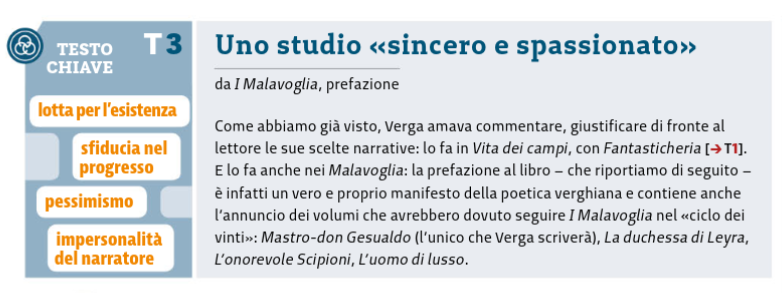
\includegraphics[width=0.75\textwidth]{./graphs/uno-studio-sincero-e-spassionato.png}
\\
\textbf{Analisi del testo}
\\
\\
Dalla marea ai vinti
\\
In un paio d'anni, il progetto originale di Verga riguardo a un ciclo di romanzi intitolato "Marea" ha subito cambiamenti. Il titolo complessivo è stato abbandonato, e ora Verga si concentra sui "vinti che levano le braccia disperate". Nella prima edizione del romanzo, il titolo "I Malavoglia" è stampato sotto questo nuovo titolo collettivo: "I vinti". L'attenzione si sposta dalle dinamiche degli eventi, simboleggiate dal mare che tutto copre, alle vittime di quegli eventi, gli uomini che le onde travolgono. L'immagine della "marea" legata ai bisogni più volgari dell'uomo viene sostituita da quella della "fiumana del progresso", che, se osservata da lontano, maschera tali bisogni trasformandoli in virtù.
\\
\\
Il pessimismo di Verga
\\
Verga cambia il titolo del terzo romanzo pianificato, da "La duchessa delle Gargantas" a "La duchessa di Leyra". Tuttavia, la struttura complessiva della serie rimane invariata, così come il pessimismo e la mancanza di fiducia nella possibilità di trovare un significato nell'incessante attività umana. Verga esprime la convinzione che i "vincitori d'oggi" saranno superati domani. Utilizza un aforisma di Kafka per illustrare il sentimento di cercare di capire il motivo dietro l'incessante attività umana, suggerendo che, come nel caso del millepiedi, la ricerca potrebbe portare solo al fallimento.
\\
\\
Gli "Interessi particolari" nella lotta per l'esistenza
\\
Nella prefazione, Verga riassume brevemente l'argomento dei "Malavoglia" evidenziando le prime inquietudini verso il benessere, con padron ’Ntoni che decide di dedicarsi al commercio di lupini. Presenta anche i romanzi successivi come una progressione ascendente, rappresentando cambiamenti nei ranghi sociali, ambizioni e ricchezze. Tuttavia, sottolinea che tutti i personaggi sono spinti dagli stessi "interessi particolari" come avidità, egoismo e ambizione. Afferma che nessuno è innocente nella lotta per l'esistenza, né i vincitori né i vinti, adottando una visione relativistica senza valori saldi. Verga esprime una visione decisamente pessimistica del progresso, suggerendo che la marcia trionfale dell'umanità si traduce in uno schiacciamento di tutti gli esseri umani agli ingranaggi della Storia.
\\
\\
Lo scrittore, un semplice testimone
\\
Verga adotta uno stile asciutto e freddo, enfatizzando l'importanza della veridicità nel suo "studio sincero e spassionato". Si ritrae come un pittore che dipinge dal vero, cercando di rappresentare la realtà con colori adatti. Questo approccio riflette l'influenza del Naturalismo di Zola, dove l'osservazione asettica è fondamentale e i sentimenti sono esclusi. Tuttavia, a differenza dei naturalisti che credevano che la letteratura potesse migliorare la società, Verga vede lo scrittore come un testimone passivo, incapace di cambiare le leggi che regolano la natura e la storia umana. Il ruolo dello scrittore, secondo Verga, è essere uno scrupoloso testimone veritiero di una tragedia, senza la capacità di influenzare significativamente la società.
\\
\newpage
\\

\includegraphics[width=0.75\textwidth]{./graphs/padronntoni.png}
\\
\\
Il brano può essere suddiviso in tre sequenze narrative. La prima colloca la famiglia Malavoglia nell'ambiente della campagna catanese, sottolineando la loro appartenenza immutata a questo contesto nel tempo. La seconda sequenza descrive i membri della famiglia sotto il comando di padron ’Ntoni, uniti come le dita di una mano. La terza allude al rispetto guadagnato dalla famiglia nel paese grazie alla sua fedeltà a una rigorosa disciplina.
\\
\\
Il narratore adotta un tono colloquiale, vicino al parlato, utilizzando parole e modi di dire tipici del dialetto siciliano. Rappresenta sé stesso come un membro anonimo della comunità di Aci Trezza, rivolgendosi ad altri membri che presumibilmente conoscono già la strada vecchia di Trezza e i luoghi menzionati.
\\
\\
Contrariamente a altri romanzi dell'Ottocento, i personaggi non vengono descritti dettagliatamente alla loro introduzione, ma emergono gradualmente nel corso del racconto, arricchendo la loro personalità. Verga cerca di creare un'illusione completa della realtà, introducendo i personaggi come se fossero già noti al lettore, rendendo così il racconto più coinvolgente e realistico.
\\
\\
La voce popolare è evidente nell'uso di discorso diretto e indiretto libero nel periodo conclusivo, dove si mescolano le parole di padron ’Ntoni e del narratore o della comunità di Aci Trezza. La tecnica narrativa di Verga mira a coinvolgere il lettore nella vita quotidiana della comunità, sottolineando l'importanza della voce popolare nel racconto.
\\

\includegraphics[width=0.78\textwidth]{./graphs/affaredeilupini.png}
\\
Il brano inizia descrivendo la tempesta che si abbatterà sulla famiglia Malavoglia, in particolare a causa della partenza di ’Ntoni per la leva militare. Questo evento rompe l'equilibrio economico precario della famiglia, portando padron ’Ntoni a assumere lavoranti a giornata, ma senza riuscire a far quadrare i conti. Cambiano i costumi della comunità, e Mena è in età da marito.
\\
\\
Successivamente, Verga introduce la crisi attraverso la narrazione dell'affare dei lupini. Zio Crocifisso vende un carico di lupini a padron ’Ntoni, nonostante siano "un po' avariati." Nonostante le perplessità della Longa, l'affare viene concluso grazie all'intervento di Piedipapera, il sensale. La Provvidenza, la barca della famiglia, parte in mare, ma la conclusione è tragica poiché la barca va a picco.
\\
\\
La sequenza si conclude con una frase che preannuncia il naufragio imminente della barca, evidenziando il tono rapido e poco patetico della narrazione. La chiusa del capitolo anticipa la tragedia imminente, seguendo la poetica verista di Verga che mira a offrire un'analisi fredda delle vicende umane senza cercare di emozionare il lettore.
\\

\includegraphics[width=0.76\textwidth]{./graphs/addiodintoni.png}
\\
Il brano inizia descrivendo la tempesta che si abbatterà sulla famiglia Malavoglia, in particolare a causa della partenza di ’Ntoni per la leva militare. Questo evento rompe l'equilibrio economico precario della famiglia, portando padron ’Ntoni a assumere lavoranti a giornata, ma senza riuscire a far quadrare i conti. Cambiano i costumi della comunità, e Mena è in età da marito.
\\
\\
Successivamente, Verga introduce la crisi attraverso la narrazione dell'affare dei lupini. Zio Crocifisso vende un carico di lupini a padron ’Ntoni, nonostante siano "un po' avariati." Nonostante le perplessità della Longa, l'affare viene concluso grazie all'intervento di Piedipapera, il sensale. La Provvidenza, la barca della famiglia, parte in mare, ma la conclusione è tragica poiché la barca va a picco.
\\
\\
La sequenza si conclude con una frase che preannuncia il naufragio imminente della barca, evidenziando il tono rapido e poco patetico della narrazione. La chiusa del capitolo anticipa la tragedia imminente, seguendo la poetica verista di Verga che mira a offrire un'analisi fredda delle vicende umane senza cercare di emozionare il lettore.

% chapter La seconda metà dell'ottocento (end)
\newpage
\chapter{Bibliografia e Sitografia} % (fold)
\label{chap:Bilbiografia e Sitografia}
\section{La seconda metà dell'ottocento}

 \href{https://www.youtube.com/watch?v=A_xK1W5Q2xU}{Positivismo e Naturalismo francese, 2020. \ https://www.youtube.com/watch?v=A_xK1W5Q2xU}

% chapter Bilbiografia e Sitografia (end)

\end{document}
